%% Run LaTeX on this file several times to get Table of Contents,
%% cross-references, and citations.

\documentclass[11pt]{book}
\usepackage{gvv}
\usepackage{gvv-book-bkup}
%\usepackage{Wiley-AuthoringTemplate}
\usepackage[sectionbib,authoryear]{natbib}% for name-date citation comment the below line
%\usepackage[sectionbib,numbers]{natbib}% for numbered citation comment the above line

%%********************************************************************%%
%%       How many levels of section head would you like numbered?     %%
%% 0= no section numbers, 1= section, 2= subsection, 3= subsubsection %%
\setcounter{secnumdepth}{3}
%%********************************************************************%%
%%**********************************************************************%%
%%     How many levels of section head would you like to appear in the  %%
%%				Table of Contents?			%%
%% 0= chapter, 1= section, 2= subsection, 3= subsubsection titles.	%%
\setcounter{tocdepth}{2}
%%**********************************************************************%%
\setcounter{tocdepth}{3}
%\includeonly{ch01}
\makeindex

\begin{document}

\frontmatter
%%%%%%%%%%%%%%%%%%%%%%%%%%%%%%%%%%%%%%%%%%%%%%%%%%%%%%%%%%%%%%%%
%% Title Pages
%% Wiley will provide title and copyright page, but you can make
%% your own titlepages if you'd like anyway
%% Setting up title pages, type in the appropriate names here:

\booktitle{OLYMPIAD Math}

\subtitle{Made Simple}

\AuAff{G. V. V. Sharma}

%% \\ will start a new line.
%% You may add \affil{} for affiliation, ie,
%\authors{Robert M. Groves\\
%\affil{Universitat de les Illes Balears}
%Floyd J. Fowler, Jr.\\
%\affil{University of New Mexico}
%}

%% Print Half Title and Title Page:
%\halftitlepage
\titlepage

%%%%%%%%%%%%%%%%%%%%%%%%%%%%%%%%%%%%%%%%%%%%%%%%%%%%%%%%%%%%%%%%
%%Copyright Page

\begin{copyrightpage}{2023}
%Title, etc
\end{copyrightpage}

% Note, you must use \ to start indented lines, ie,
% 
% \begin{copyrightpage}{2004}
% Survey Methodology / Robert M. Groves . . . [et al.].
% \       p. cm.---(Wiley series in survey methodology)
% \    ``Wiley-Interscience."
% \    Includes bibliographical references and index.
% \    ISBN 0-471-48348-6 (pbk.)
% \    1. Surveys---Methodology.  2. Social 
% \  sciences---Research---Statistical methods.  I. Groves, Robert M.  II. %
% Series.\\

% HA31.2.S873 2004
% 001.4'33---dc22                                             2004044064
% \end{copyrightpage}

%%%%%%%%%%%%%%%%%%%%%%%%%%%%%%%%%%%%%%%%%%%%%%%%%%%%%%%%%%%%%%%%
%% Only Dedication (optional) 

%\dedication{To my parents}

\tableofcontents

%\listoffigures %optional
%\listoftables  %optional

%% or Contributor Page for edited books
%% before \tableofcontents

%%%%%%%%%%%%%%%%%%%%%%%%%%%%%%%%%%%%%%%%%%%%%%%%%%%%%%%%%%%%%%%%
%  Contributors Page for Edited Book
%%%%%%%%%%%%%%%%%%%%%%%%%%%%%%%%%%%%%%%%%%%%%%%%%%%%%%%%%%%%%%%%

% If your book has chapters written by different authors,
% you'll need a Contributors page.

% Use \begin{contributors}...\end{contributors} and
% then enter each author with the \name{} command, followed
% by the affiliation information.

% \begin{contributors}
% \name{Masayki Abe,} Fujitsu Laboratories Ltd., Fujitsu Limited, Atsugi, Japan
%
% \name{L. A. Akers,} Center for Solid State Electronics Research, Arizona State University, Tempe, Arizona
%
% \name{G. H. Bernstein,} Department of Electrical and Computer Engineering, University of Notre Dame, Notre Dame, South Bend, Indiana; formerly of
% Center for Solid State Electronics Research, Arizona
% State University, Tempe, Arizona 
% \end{contributors}

%%%%%%%%%%%%%%%%%%%%%%%%%%%%%%%%%%%%%%%%%%%%%%%%%%%%%%%%%%%%%%%%
% Optional Foreword:

%\begin{foreword}
%\lipsum[1-2]
%\end{foreword}

%%%%%%%%%%%%%%%%%%%%%%%%%%%%%%%%%%%%%%%%%%%%%%%%%%%%%%%%%%%%%%%%
% Optional Preface:

%\begin{preface}
%\lipsum[1-1]
%\prefaceauthor{}
%\where{place\\
% date}
%\end{preface}

% ie,
% \begin{preface}
% This is an example preface.
% \prefaceauthor{R. K. Watts}
% \where{Durham, North Carolina\\
% September, 2004}

%%%%%%%%%%%%%%%%%%%%%%%%%%%%%%%%%%%%%%%%%%%%%%%%%%%%%%%%%%%%%%%%
% Optional Acknowledgments:

%\acknowledgments
%\lipsum[1-2]
%\authorinitials{I. R. S.}  

%%%%%%%%%%%%%%%%%%%%%%%%%%%%%%%%
%% Glossary Type of Environment:

% \begin{glossary}
% \term{<term>}{<description>}
% \end{glossary}

%%%%%%%%%%%%%%%%%%%%%%%%%%%%%%%%
%\begin{acronyms}
%\acro{ASTA}{Arrivals See Time Averages}
%\acro{BHCA}{Busy Hour Call Attempts}
%\acro{BR}{Bandwidth Reservation}
%\acro{b.u.}{bandwidth unit(s)}
%\acro{CAC}{Call / Connection Admission Control}
%\acro{CBP}{Call Blocking Probability(-ies)}
%\acro{CCS}{Centum Call Seconds}
%\acro{CDTM}{Connection Dependent Threshold Model}
%\acro{CS}{Complete Sharing}
%\acro{DiffServ}{Differentiated Services}
%\acro{EMLM}{Erlang Multirate Loss Model}
%\acro{erl}{The Erlang unit of traffic-load}
%\acro{FIFO}{First in - First out}
%\acro{GB}{Global balance}
%\acro{GoS}{Grade of Service}
%\acro{ICT}{Information and Communication Technology}
%\acro{IntServ}{Integrated Services}
%\acro{IP}{Internet Protocol}
%\acro{ITU-T}{International Telecommunication Unit -- Standardization sector}
%\acro{LB}{Local balance}
%\acro{LHS}{Left hand side}
%\acro{LIFO}{Last in - First out}
%\acro{MMPP}{Markov Modulated Poisson Process}
%\acro{MPLS}{Multiple Protocol Labeling Switching}
%\acro{MRM}{Multi-Retry Model}
%\acro{MTM}{Multi-Threshold Model}
%\acro{PASTA}{Poisson Arrivals See Time Averages}
%\acro{PDF}{Probability Distribution Function}
%\acro{pdf}{probability density function}
%\acro{PFS}{Product Form Solution}
%\acro{QoS}{Quality of Service}
%\acro{r.v.}{random variable(s)}
%\acro{RED}{random early detection}
%\acro{RHS}{Right hand side}
%\acro{RLA}{Reduced Load Approximation}
%\acro{SIRO}{service in random order}
%\acro{SRM}{Single-Retry Model}
%\acro{STM}{Single-Threshold Model}
%\acro{TCP}{Transport Control Protocol}
%\acro{TH}{Threshold(s)}
%\acro{UDP}{User Datagram Protocol}
%\end{acronyms}

\setcounter{page}{1}

\begin{introduction}
This book links high school coordinate geometry to linear algebra and matrix analysis through solved problems.

\end{introduction}

\mainmatter
%\chapter{Vectors}
%\section{2020}
%\subsection{10}
%\begin{enumerate}
\item The distance between the points $\brak{m,-n}$ and $\brak{-m, n}$ is
\begin{enumerate}
\item $\sqrt{m^{2} + n^{2}}$
\item $ m+n $
\item $ 2\sqrt{m^{2} + n^{2}}$
\item $\sqrt{2m^{2} + 2n^{2}}$
\end{enumerate}
\item The point on the x-axis which is equidistant from $\brak{-4,0}$ and $\brak{10,0}$ is
\begin{enumerate}             
\item $\brak{7,0}$
\item $\brak{5,0}$              
\item $\brak{0,0}$
\item $\brak{3,0}$
\end{enumerate}
\item The centre of a circle whose end points of a diameter are $\brak{-6,3}$ and $\brak{6,4}$ is
\begin{enumerate}
\item $\brak{8,-1}$
\item $\brak{4,7}$
\item $\brak{0,\frac{7}{2}}$
\item $\brak{4,\frac{7}{2}}$
\end{enumerate}
\item $AOBC$ is a rectangle whose three vertices are $\vec{A}\brak{0,-3}$, $\vec{O}\brak{0,0}$ and $\vec{B}\brak{4,0}$. The length of its diagonal is $\rule{3cm}{0.15mm}$.
\item Find the ratio in which the $y-axis$ divides the line segment joining the points $\brak{6,-4}$ and $\brak{-2, -7}$. Also find the point of intersection.
\item Show that the points $\brak{7, 10}$, $\brak{-2, 5}$ and $\brak{3, 4}$ are vertices of an isosceles right triangle.
\end{enumerate}

%\subsection{12}
%
\begin{enumerate}
\item The area of a triangle formed by vertices $\vec{O}$, $\vec{A}$ and $\vec{B}$, where $\overrightarrow{OA}= \hat{i}+2 \hat{j}+3\hat{k}$ and $\overrightarrow{OB}= -3\hat{i} - 2\hat{j} + \hat{k}$ is
\begin{enumerate}
\item $3\sqrt{5}$ sq. units
\item $5\sqrt{5}$ sq. units
\item $6\sqrt{5}$ sq. units
\item $4$ sq. units
\end{enumerate}
\item The coordinates of the foot of the perpendicular drawn from the point $\brak{2,-3,4}$ on the $y-axis$ is
\begin{enumerate}
\item $\brak{2, 3, 4}$
\item $\brak{-2,-3,-4}$
\item $\brak{0,-3, 0}$
\item $\brak{2, 0,4}$
\end{enumerate}
\item The angle between the vectors $\hat{i} - \hat{j}$ and $\hat{j} - \hat{k}$ is
\begin{enumerate}
\item $\frac{-\pi}{3}$
\item $0$
\item $\frac{\pi}{3}$
\item $\frac{2\pi}{3}$
\end{enumerate}
\item If $\mydet{\overrightarrow{a}}= 4$ and $-3 \leq \lambda \leq 2$, then $\mydet{\lambda \overrightarrow a}$ lies in
\begin{enumerate}
\item $\sbrak{0,12}$
\item $\sbrak{2,3}$
\item $\sbrak{8,12}$
\item $\sbrak{-12,8}$
\end{enumerate}
\item The distance between parallel planes $2x + y - 2z - 6 = 0$ and $4x + 2y - 4z = 0$ is $\rule{3cm}{0.15mm}$ units.
\item If $\vec{P}\brak{1,  0, -3}$ is the foot of the perpendicular from the origin to the plane, then the cartesian equation of the plane is $\underline{\hspace{3cm}}$.
\item Find the coordinates of the point where the line $\frac{x-1}{3} = \frac{y+4}{7} = \frac{z+4}{2}$ cuts the $xy-plane$.
\item Find a vector $\overrightarrow{r}$ equally inclined to the three axes and whose magnitude is $3\sqrt{3}$ units.
\item Find the angle between unit vectors $\overrightarrow{a}$ and $\overrightarrow{b}$ so that $\sqrt{3}\overrightarrow{a}$ - $\overrightarrow{b}$ is also a unit vector.
\item Show that the plane $x - 5y - 2z = 1$ contains the line $\frac{x - 5}{3}$ = y = $2 -z$.
\item Find the equation of the plane passing through the points $\brak{1, 0, -2}$,  $\brak{3, -1, 0}$ and perpendicular to the plane $2x - y + z = 8$. Also find the distance of the plane thus obtained from the origin.
\end{enumerate}





\chapter{Linear Forms}
%\section{2023}
%\subsection{10}
%
\begin{enumerate}



  \item \textbf{Assertion (A):} Point $\vec{P}$(0,2) is the point of intersection of $y-axis$ with  the line $3x+2y=4$.\\
    \textbf{Reason (R):} The distance of point $\vec{P}$(0,2) from $x-axis$ is 2 units.


  \item If the pair of equations $3x-y+8=0$ and $6x-ry+16=0$ represent coincident lines, then the value of \text{'$r$'} is:

    \begin{enumerate}
      \item $-\frac{1}{2}$
      \item $\frac{1}{2}$
      \item -2
      \item 2
    \end{enumerate}

  \item The of linear equations $2x=5y+6$ and $15y=6x-18$ represents two lines which are:

      \begin{enumerate}
        \item intersecting
        \item parallel
        \item coincident
        \item either intersecting or parallel
      \end{enumerate}

    \item Find the equations of the diagonals of the parallelogram $\vec{PQRS}$ whose vertices are $\vec{P}$(4,2,-6), $\vec{Q}$(5,-3,1), $\vec{R}$(12,4,5) and $\vec{S}$(11,9,-2). Use these equations to find the point of intersection of diagonals.

  \item A line $l$ passes through point (-1,3,-2) and is perpendicular to both the lines $\frac {x}{1}=\frac{y}{2}=\frac{z}{3}$ and $\frac {x+2}{-3}=\frac{y-1}{2}=\frac{z+1}{5}$. Find the ctor equation of the line $l$. Hence, obtain its distance from origin.

\end{enumerate}

%\subsection{12}                                                                                                  
%\begin{enumerate}
    \item Equation of line passing through origin and making $30\degree,60\degree$ and $90\degree$ with $x,y,z$ axes respectively is
    \begin{enumerate}
        \item $\frac{2x}{\sqrt3}=\frac{y}{2}=\frac{z}{0}$
        \item $\frac{2x}{\sqrt3}=\frac{2y}{1}=\frac{z}{0}$
        \item $2x=\frac{2y}{\sqrt3}=\frac{z}{1}$
        \item $\frac{2x}{\sqrt3}=\frac{2y}{1}=\frac{z}{1}$
    \end{enumerate}
    \item If the equation of a line is $x=ay+b,z=cy+d$,then find the direction ratios of the line and a point on the line.
    \item
    \begin{enumerate}
        \item Find the equations of the diagonals of the parallelogram $PQRS$ whose vertices are$P(4,2,-6),Q(5,-3,1),R(12,4,5),S(11,9,-2)$.Use these equations to find the point of intersection of diagonals.  
        \item A line $l$ passes through point$(-1,3,-2)$ and is perpendicular to both the lines $\frac{x}{1}=\frac{y}{2}=\frac{z}{3}$ and $\frac{x+2}{-3}=\frac{y-1}{2}=\frac{z+1}{5}$.Find the vector equation of the line $l$.Hence,obtain its distance from origin.
    \end{enumerate}
   
   
   
\end{enumerate}


%\section{2022}

\chapter{Circles}
\begin{enumerate}
	\item In tangents $\vec{PA}$ and $\vec{PB}$ from an external point $P$ to a circle with centre $O$ , are inclined to each other at an angle of $80^{\degree}$, then $\angle AOB$ is equal to
 \begin{figure}[H]
        \centering
        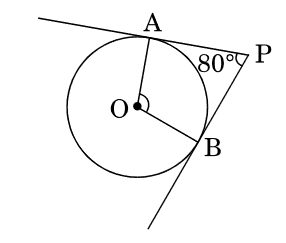
\includegraphics[width = \columnwidth]{figs/Tan_circle23.png}
        \caption{Tangents $PA$ and $PB$}
        \label{fig:Tan_circle23}
    \end{figure}
    \begin{enumerate}
        \item $100^{\degree}$
        \item $60^{\degree}$
        \item $80^{\degree}$
        \item $50^{\degree}$
    \end{enumerate}

    \item  Two concentric circles are of radii $4 cm$ and $3 cm$. Find the length of the chord of the larger circle which touches the smaller circle.

    \item  In a triangle $ABC$ with $\angle AOB$ is shown. Taking $AB$ as diameter, a circle has been drawn intersecting $AC$ at point $P$. Prove that the tangent drawn at point $P$ bisects $BC$. 
	    \begin{figure}[H]
            \centering
                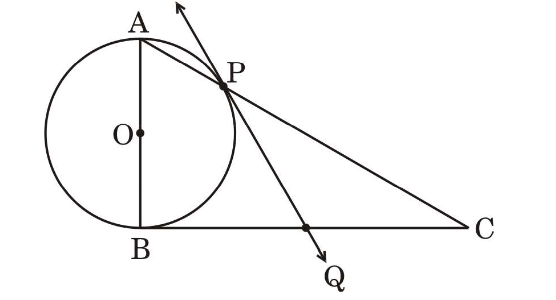
\includegraphics[width = \columnwidth]{figs/concen_circle23.png}
                \caption{Concentric circles}
                \label{fig:concen_circle23}
        \end{figure}
    \item  Prove that a Parallelogram circumscribing a circle is a rhombus.
     \item  In two circles with centres at $O$ and $O$ of radii $2r$ and $r$ respectively, touch each other internally at $A$. A chord $AB$ of the bigger circle meets the smaller circle at $C$. Show that  $C$ bisects $AB$.
    \begin{figure}[H]
        \centering
        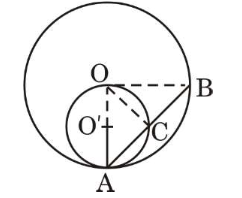
\includegraphics[width = \columnwidth]{figs/two_circle23.png}
        \caption{Two circles with center}
        \label{fig:two_circle23}
    \end{figure}  
    
    \item In $O$ is centre of a circle of radius $5 cm$. $PA$ and $BC$ are tangents to the circle at $A$ and $B$ respectively. If $OP = 13 cm$, then find the length of tangents $PA$ and $BC$.
\begin{figure}[H]                                                                                             
\centering                                                                                                
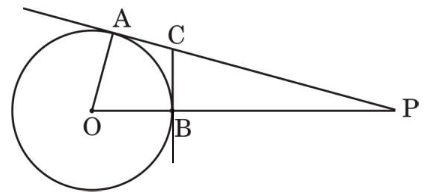
\includegraphics[width = \columnwidth]{figs/circle_radius23.png}
\caption{The center of circle radius is $5m$}
	\label{fig:circle_radius23}        
\end{figure}

    \item In two concentric circles, a chord of length $48 cm$ of the larger
circle is a tangent to the smaller circle, whose radius is $7 cm$. Find the radius of the larger circle. 
    \item At a point on the level ground, the angle of elevation of the top
of a vertical tower is found to be $\alpha$, such that $\tan \alpha =\frac{5}{12} $. On walking $192 m$ towards the tower, the angle of elevation $\beta$ is such that $\tan \beta=\frac{3}{4}$. Find the height of the tower. 
\end{enumerate}

%\section{2010}
%\subsection{12}
%\begin{enumerate}
	\item In tangents $\vec{PA}$ and $\vec{PB}$ from an external point $P$ to a circle with centre $O$ , are inclined to each other at an angle of $80^{\degree}$, then $\angle AOB$ is equal to
 \begin{figure}[H]
        \centering
        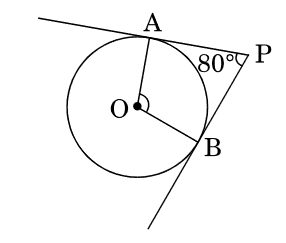
\includegraphics[width = \columnwidth]{figs/Tan_circle23.png}
        \caption{Tangents $PA$ and $PB$}
        \label{fig:Tan_circle23}
    \end{figure}
    \begin{enumerate}
        \item $100^{\degree}$
        \item $60^{\degree}$
        \item $80^{\degree}$
        \item $50^{\degree}$
    \end{enumerate}

    \item  Two concentric circles are of radii $4 cm$ and $3 cm$. Find the length of the chord of the larger circle which touches the smaller circle.

    \item  In a triangle $ABC$ with $\angle AOB$ is shown. Taking $AB$ as diameter, a circle has been drawn intersecting $AC$ at point $P$. Prove that the tangent drawn at point $P$ bisects $BC$. 
	    \begin{figure}[H]
            \centering
                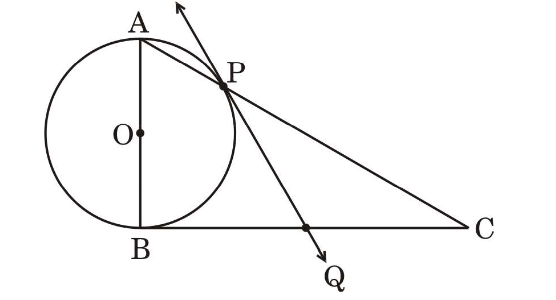
\includegraphics[width = \columnwidth]{figs/concen_circle23.png}
                \caption{Concentric circles}
                \label{fig:concen_circle23}
        \end{figure}
    \item  Prove that a Parallelogram circumscribing a circle is a rhombus.
     \item  In two circles with centres at $O$ and $O$ of radii $2r$ and $r$ respectively, touch each other internally at $A$. A chord $AB$ of the bigger circle meets the smaller circle at $C$. Show that  $C$ bisects $AB$.
    \begin{figure}[H]
        \centering
        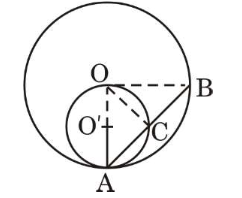
\includegraphics[width = \columnwidth]{figs/two_circle23.png}
        \caption{Two circles with center}
        \label{fig:two_circle23}
    \end{figure}  
    
    \item In $O$ is centre of a circle of radius $5 cm$. $PA$ and $BC$ are tangents to the circle at $A$ and $B$ respectively. If $OP = 13 cm$, then find the length of tangents $PA$ and $BC$.
\begin{figure}[H]                                                                                             
\centering                                                                                                
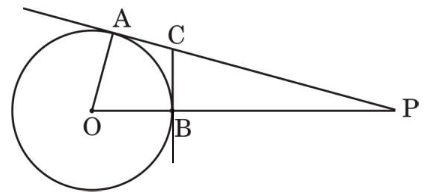
\includegraphics[width = \columnwidth]{figs/circle_radius23.png}
\caption{The center of circle radius is $5m$}
	\label{fig:circle_radius23}        
\end{figure}

    \item In two concentric circles, a chord of length $48 cm$ of the larger
circle is a tangent to the smaller circle, whose radius is $7 cm$. Find the radius of the larger circle. 
    \item At a point on the level ground, the angle of elevation of the top
of a vertical tower is found to be $\alpha$, such that $\tan \alpha =\frac{5}{12} $. On walking $192 m$ towards the tower, the angle of elevation $\beta$ is such that $\tan \beta=\frac{3}{4}$. Find the height of the tower. 
\end{enumerate}



\chapter{Intersection of Conics}

%\section{2010}
%\subsection{12}
%\input{2010/intersec.tex}





\chapter{Probability}
%\section{chapters}


\begin{enumerate}
	\item Probability of happining of an event is denoted by $p$ and probability of non-happening of the event is denoted by $q$. Relation between $p$ and $q$ is
                        \begin{enumerate}
                                \item $p$+$q$=1
                                \item $p$=1, $q$=1
                                \item $p$=$q$-1
                                \item $p$+$q$+1=0
                        \end{enumerate}
			
        \item A girl calculates that the probability of her winning the first prize in a lottery is 0.08. If 6000 tickets are sold, how many tickets has she bought ?
                        \begin{enumerate}
                                \item  40
                                \item  240
                                \item  480
                                \item  750

                        \end{enumerate}
        \item In a group of 20 people, 5 can't swim. If one person is selected at random, then the probability that he/sh can swim, is
                        \begin{enumerate}
                                \item $ \frac {3} {4} $
                                \item $ \frac {1} {3} $
                                \item 1
                                \item $ \frac {1} {4} $
                        \end{enumerate}
        \item A bag contain 4 red, 3 blue and 2 yellow balls. One ball is drawn at random from the bag. Find the probability that drawn ball is
                \begin{enumerate}[(i)]
                                        \item red
                                        \item yellow
                \end{enumerate}
        \item A bag contain 100 cards numbered 1 to 100.Acard is drawn at random from the b. What is the probability that the number on the card is a perfect cube ?
                        \begin{enumerate}
                                \item $ \frac {1} {20} $
                                \item $ \frac {3} {50} $
                                \item $ \frac {1} {25} $
                                \item $ \frac {7} {100} $
                        \end{enumerate}
        \item If three coins are tossed simultaneously, what is the probability of getting a most one trail ?
                        \begin{enumerate}
                                \item $ \frac {3} {8} $
                                \item $ \frac {4} {8} $
                                \item $ \frac {5} {8} $
                                \item $ \frac {7} {8} $
                        \end{enumerate}
        \item Two dics are thrown together. The probability of getting the difference of numbers on their upper faces equals to 3 is :
                        \begin{enumerate}
                                \item $ \frac {1} {9} $
                                \item $ \frac {2} {9} $
                                \item $ \frac {1} {6} $
                                \item $ \frac {1} {12} $
                        \end{enumerate}
        \item A card is drawn at random from a well-shuffled pack of 52 cards. The probability that the card drawn is not an ace is :

                        \begin{enumerate}
                                \item $ \frac {1} {13} $
                                \item $ \frac {9} {13} $
                                \item $ \frac {4} {13} $
                                \item $ \frac {12} {13} $
                        \end{enumerate}
        \item \textbf{Assertion (A) : } The probability that a leap year has 53 Students is $ \frac {2} {7} $.\\
                \textbf{Reason (R) : } The probability that a non-leap year has 53 Sundays is $ \frac {5} {7} $.

                          \begin{enumerate}
                                  \item Both Assertion (A) and Reason (R) are true and Reason (R) is the correct explanation of Assertion (A).
                                  \item Both Assertion (A) and Reason (R) are true and Reason (R) is not the correct explanation of Assertion (A).
                                  \item Assertion (A) is true but Reason (R) is false.
                                  \item Assertion (A) is false but Reason (R) is true.
                          \end{enumerate}


\end{enumerate}
\end{document}

%\section{chapters}
\begin{enumerate}
\item A postman has to deliver ive letters to five different houses. Mischievously, he posts one letter through each door without looking to see if it is the correct address. In how rnany different way could he do this so that exactly two of the five houses receive the correct letters?\hfill(PRERMO 2012)
\end{enumerate}


\chapter{permutation and combination}
%\section{chapters}
\begin{enumerate}
	\item A positive integer $n > 1$ is called beautiful if $n$ can be written in one and only one way as $n = a_{1} + a_{2} + \cdots + a_{k} = a_{1} \cdot a_{2} \cdots a_{k} $for some positive integers $a_{1},a_{2}, \cdots , a_{k}$ , where $k > 1$ and$ a_{1}  \geq a_{2} \geq \cdots \geq a_{k}$ . (For example $6$ is beautiful since$ 6 = 3 \cdot 2 \cdot 1 = 3 + 2 + 1$ , and this is unique. But $8$ is not beautiful since $8 = 4 + 2 + 1 + 1 = 4 \cdot 2 \cdot 1 \cdot 1 $  as well as $8 = 2 + 2 + 2 + 1 + 1 = 2 \cdot 2 \cdot 2 \cdot 1 \cdot 1$ , souniqueness is lost.) Find the largest beautiful number less than $100$.\hfill(IOQM 2015)



	\item For $n \in N$ , consider non-negative integer-valued functions $f$ on $\cbrak{1, 2, \cdots , n}$ satisfying $f\brak{i} \geq f\brak{j}$ for $i > j$ and $\sum_{i=1}^n \brak{i + f\brak{i}} = 2023$ . Choose $n$ such that $\sum_{i=1}^n f\brak{i}$ is the least. How many such functions exist in that case?\hfill(IOQM 2015)



	\item In the land of Binary, the unit of currency is called Ben and currency notes areavailable in denominations $1, 2, 2^2, 2^3, \cdots $ Bens. The rules of the Government of Binary stipulate that one can not use more than two notes of any one denomination in any transaction. For example, one can give a change for $2$ Bens in two ways: $2$ one Ben notes or $1$ two Ben note. For $5$ Ben one can give $1$ one Ben note and $1$ four Ben note or $1$ one Ben note and $2$ two Ben notes. Using $5$ one Ben notes or $3$ one Ben notes and $1$ two Ben notes for a $5$ Ben transaction is prohibited. Find the number of ways in which one can give change for $100$ Bens, following the rules of the Government.\hfill(IOQM 2015)	
	\item Unconventional dice are to be designed such that the six faces are marked with numbers from $1$ to $6$ with $1$ and $2$ appearing on opposite faces. Further, each face is colored either red or yellow with opposite faces always of the same color. Two dice are considered to have the same design if one of them can be rotated to obtain a die that has the same numbers and colors on the corresponding faces as the other one. Find the number of distinct dice that can be designed.\hfill(IOQM 2015)
    
	\item Given a $2 \times 2$ tile and seven dominoes ($2 \times 1$ tile), find the number of ways of tiling a $2 \times 7$ rectangle using some of these tiles.\hfill(IOQM 2015)
    
    \item Consider the set 
	    \begin{align}
		    S = \cbrak{\brak{a, b, c, d, e} : 0 < a < b < c < d < e < 100}
	    \end{align}
\\where $a, b, c, d, e$ are integers. If $D$ is the average value of the fourth element of such a tuple in the set, taken over all the elements of $S$, find the largest integer less than or equal to $D$.\hfill(IOQM 2015)
    
    \item Let $P$ be a convex polygon with $50$ vertices. A set $F$ of diagonals of $P$ is said to be minimally friendly if any diagonal $d \in F$ intersects at most one other diagonal in $F$ at a point interior to $P$. Find the largest possible number of elements in a minimally friendly set $F$.\hfill(IOQM 2015)
    \item Find all pairs $(k, n)$ of positive integers such that
\begin{align}
k! = \brak{2n - 1}\brak{2n - 2}\brak{2n - 4} \cdots \brak{2n - 2n + 1}.
\end{align}
\hfill(IMO 2019)
\item There are 4n pebbles of weights 1,2,3.....,4n.Each pebble is coloured in one of n colours and there are four pebbles of each colour.Show that we can arrange the pebbles into two piles so that the following two conditions are both satisfied:

    The total weights of both piles are the same.
    Each pile contains two pebbles of each colour.
\hfill(IMO 2020)
\item Two squirrles,Bushy and jumpy,have collected 2021 walnuts for the winter .jumpy  numbers the walnuts from 1 through 2021,and digs 2021 little holes in a circular pattern in the ground around their favourite tree.The next morning jumpy notices that bushy had placed one walnut into each hole ,but had paid no attention to the numbering .unhappy,Jumpy decides to reorder the walnuts by performing a sequence of 2021 moves.In the k-th move,jumpy swaps the positions of the two walnuts adjacent to walnut k.Prove that there exists a value of k such that ,on the k-th move,jumpy swaps some walnuts a and b such that $a< k< b$.
\hfill(IMO 2021)
\item Twenty-one girls and twenty-one boys took part in a mathematical contest. Each contestant solved a t most six problems. For each girl and each boy, at least one problem was solved by both of them. Prove t hat there was a problem that was solved by at least three girls and at least three boys. \hfill(IMO 2001 )
\item $S$ is the set $\{1,2,3,\ldots, 1000000 \}$. Show that for any subset $A$ of $S$ with $101$ elements we can find $100$ distinct elements $x_{i}$ of $S$, such that the sets $\{a+x_{i} a\in A\}$ are all pairwise disjoint.\hfill(IMO 2003)
\item $S$ is the set of all $\brak{h, k}$ wi th $h$, $k$ non-negative integers such that $h + k \ textless n$. Each element of $S$ is colored red or b lue, so that if \brak{h, k} is red and $h'\leq h,k'\ leq k$, then $\brak{h', k'}$ is also red. $A$ type $ 1$ subset of $S$ has $n$ blue elements with differen t first member and a type $2$ subset of $S$ has $n$ blue elements with different second member. Show tha t there are the same number of type $1$ and type $2$ subsets.\hfill (IMO 2002)
\item  To each vertex of a regular pentagon an integer is assigned in such a way that the sum of all five numbers is positive. If three consecutive vertices are assigned the numbers $x$,$y$,$z$ respectively and $y<0$ then the following operation is allowed: the numbers $x$,$y$,$z$ are replaced by $x+y$,$-y$,$z+y$ respectively. Such an operation is performed repeatedly as long as at least one of the live numbers is negative. Determine whether this procedure necessarily comes to and end after a finite number of steps.\hfill(IMO 1986)
\item One is given a finite set of points in the plane, each point having integer coordinates. Is it always possible to color some of the points in the set red and the remaining points white in such a way that for any straight line $L$ parallel to either one of the coordinate axes the difference (in absolute value) between the numbers of white point and red points on $L$ is not greater than $1$?\hfill(IMO 1986)
\item Let $x_1, x_2, \dots, x_n$ be real numbers satisfying $x^2_1 +x^2_2 +\dots+x^2_n = 1$. Prove that for every integer $k\geq2$ there are integers $a_1, a_2, \dots , a_n$, not all $0$, such that $\mydet{a_i}\leq k-1$ for all $i$ and 
                     \begin{align*} \mydet{a_1x_1+a_2x_2+\dots+a_nx_n} \leq \frac{\brak{k-1}\sqrt{n}}{k^n-1} \end{align*}\hfill(IMO 1987)
	 \item Let $n$ be an integer greater than or equal to $2$. Prove that if $k^2+k+n$ is prime for all integers $k$ such that $0\leq k\leq \sqrt{n/3}$, then $k^2+k+n$ is prime for all integers $k$ such that $0\leq k\leq n-2$ \hfill(IMO 1987)
 \item Problem 4. Let $n \geq  3$ be an integer, and consider a circle with $n+1$ equally spaced points marked on it. Consider all labellings of these points with the numbers $0,1,\    ldots n$ such that each label is used exactly once, two such labellings are considered to be the same if one can be obtained from the other by a rotation of the circle. A labelling     is called beautiful if, for any four labels $a< b<c < d$ with $a+d=b+c,$ the chord joining the points labelled $a$ and $d$ does not intersect the chord joi    ning the points labelled $b$ and $c$                                                                                                                                                                                                                                                                                                                                     Let $M$ be the number of beautiful labellings, and let $N$ be the number of ordered pairs $\brak{x, y}$ of  positive integers such that $x+y\leq n and gcd \brak{x,y} = 1$. Prove that                                                                                                                                                                                                                                                                                                                                $m=n+1$  
 \item An international society has its members from six different countries. The list of members contains $1978$ names, numbered $1, 2,\ldots$, $1978$. Prove that there is at least one member whose number is the sum of the numbers of two members from his own country, or twice as large as the number of one member from his own country.\hfill(Imo 1978)

	\item Let $A$ and $E$ be opposite vertices of a regular octagon. $A$ frog starts jumping at vertex $A$. From any vertex of the octagon except $E$, it may jump to either of the two adjacent vertices. When it reaches vertex $E$, the frog stops and stays there.. Let a be the number of distinct paths of exactly $n$ jumps ending at $E$. Prove that 
\begin{align}a_2n-1=0, a_{2n} = \frac{1}{\sqrt{2}}\brak{x^{n - 1} - y^{n - 1}}\end{align},
$n = 1, 2, 3 ,\ldots$,
	where $x = 2 + \sqrt{2}$ and $y = 2 - \sqrt{2}$ . Note. A path of a jumps is a sequence of vertices $\brak{P_0\ldots P_n}$ such that
\begin{enumerate}
	\item $PA, P = E$
\item for every $i, 0 \leq i \leq n - 1, P$ is distinct from $E$;
\item for every $i, 0 \leq i \leq n - 1 P$. and $P_{i+1}$ are adjacent.\end{enumerate}\hfill(Imo 1979)
	\subsection*{ Algebra}  
\item Find all real numbers a for which there exist non-negative real numbers $x_1, x_2, x_3, x_4,x_5$ satisfying the relations \begin{align}\sum_{k=1}^{5}kx_{k}=a,\sum{k=1}{5}k^{3}x_{k}=a^2,\sum{k=1}{5}k^{5}x_{k}=a^3\end{align}.\hfill(Imo 1979)
\item In a competition, there are $a$ contestants and $b$ judges, where $ b \geq 3$ is an odd integer. Each judge rates each contestant as either "pass" or "fail". Suppose $k$ is a number such that, for any two judges, their ratings coincide for at most $k$ contestants. Prove that $ \frac{k}{a} \geq \frac{\brak{b-1}}{\brak{2b}}$.\hfill(IMO 1998)                                                      
	
\item Consider an $n \times n$ square board, where $n$ is a fixed even positive integer.The board is divided into $n^2$ unit squares. We say that two different squares on the board are adjacent if they have a common side.$N$ unit squares on the board are marked in such a way that every square \brak{marked or unmarked} on the board is adjacent to at least one marked square.Determine the smallest possible value of $N$.\hfill(IMO 1999)
	
\item $k$ is a positive real. $N$ is an integer greater than $1$. $N$ points are placed on a line, not all coincident. $A$ $move$ is carried out as follows. Pick any two points $A$ and $B$ which are not coincident. Suppose that $A$ lies to the right of$B$.Replace $B$ by another point $B'$ to the rightof $A$ such that $AB' = kBA$. For what values of $k$ can we move the points arbitrarily far to the right by repeated moves?\hfill(IMO 2000) 

\item $100$ cards are numbered $1$ to $100$ $\brak{each card different}$ and placed in $3$ boxes $\brak{at least one card in each box}$. How many wa ys can this be done so that if two boxes are selected and a card is taken from each, then the knowledgeof their sum alone is always sufficient to identify the third box?\hfill(IMO 2000)                       
\item The equation \begin{align}(x - 1)(x - 2)....(x-2016)=(x-1)(x-2)...(x-2016)\end{align} is written on the board, with $2016$ linear factors on each side. What is the least possible value of $k$ for which it is possible to erase exactly $k$ of these $4032$ linear factors so that at least one factor remains on each side and the resulting equation has no real solutions?\hfill (IMO 2016)
 \item Let $S$ be a finite set of points in three-dimensional space. Let $S_x$, $S_y$, $S_z$ be the sets consisting of the orthogonal projections of the points of $S$ onto the $yz$-plane, $zx$-plane, $xy$- plane, respectively. Prove that    \hfill(IMO 1992)
 
$|S|^{2} \leq |S_x| \cdot |S_y| \cdot |S_z|$,
 

 where $|A|$ denotes the number of elements in the finite set $|A|$. (Note: The orthogonal projection of a point onto a plane is the foot of the perpendicular from that point to the plane.)
\item Consider nine points in space, no four of which are coplanar. Each pair of points is joined by an edge (that is, a line segment) and each edge is either coloured blue or red or left uncoloured. Findthe smallest value of $n$ such that whenever exactly $n$ edges are coloured, the set of coloured edges necessarily contains a triangle all of whose edges have the same color. \hfill(IMO 1992)
\item On an infinite chessboard, a game is played as follows. At the start, $n^{2}$ pieces are arranged on the chessboard in an $n$ by $n$ block of adjoining squares, one piece in each square. A move in the game is a jump in a horizontal or vertical direction over an adjacent occupied square to an unoccupied square immediately beyond. The piece which has  been jumped over is removed.                        
 Find those values of $n$ for which the game can end with only one piece remaining on the board.  \hfill(IMO 1993)
\item There are $n$ lamps $L_0, \dots , L_{ n-1 }$  in a circle $(n > 1) $, where we denote $L_{n+k} =  L_k$. (A lamp at all times is either on or off.) Perform steps $s_0, s_1, \dots $ as follows: at step $s_i$, if $L_{i-1}$ is lit, switch $L_i$ from on to off or vice versa, otherwise do nothing. Initially all lamps are on. Show that:            \hfill(IMO 1993)                                                  

$(a)$ There is a positive integer $M(n)$ such that     after $M(n)$ steps all the lamps are on again;                                                           

 $(b)$ If $n = 2^{k}$, we can take $M(n) = n^{2}-1$;                                                          

$(c)$ If $n = 2^{k}+1$, we can take $M(n) = n^{2}-n+1$.   

\item For any positive integer $k$, let $f(k)$ be the number of elements in the set $\{ k+1, k+2, \dot s, 2k \}$ whose base $2$ representation has precisely three $1s$.
 
   $(a)$ Prove that, for each positive integer $m$, there exists at least one positive integer $k$ such that $f(k)=m$.
 
		  $(b)$ Determine all positive integers $m$ for which there exists exactly one $k$ with $f(k)= m$.     \hfill(IMO 1994)
\end{enumerate}

%\section{2015}
 \begin{enumerate}
 \item How many line segments have both their endpoints located at the vertices of a given cube? \hfill(PRERMO 2015)

    \item Let $E(n)$ denote the sum of the even digits of $n$. For example, $ E(1243) = 2 + 4 = 6 $. What is the value of $ E(1) + E(2) + E(3) + \cdots + E(100)? $ \hfill(PRERMO 2015)

    \item At a party, each man danced with exactly four women and each woman danced with exactly three men. Nine men attended the party. How many women attended the party? \hfill(PRERMO 2015)
    \end{enumerate}

%\section{2010}
%\subsection{12}
%%Exercise 8.1 prob 47
\begin{tikzpicture}
[scale=0.5,>=stealth,point/.style={draw,circle,fill = black,inner sep=0.5pt},]
%\tikzset{shift={(-3,0)}}
%Triangle sides
\def\a{4}
\def\c{9}
\def\xA{4}
\def\h{3}
\def\k{1}
%\def\c{7.5}
\def\yE{\h/2}
%Labeling points
\node (D) at (0,0)[point,label=below left:$D$] {};
\node (B) at ({\xA+\a}, \h )[point,label=above right:$B$] {};
\node (C) at (\c, 0)[point,label=below right:$C$] {};
%\node (E) at (2, \yE)
%\node (F) at (8.5, \yE)[point,label=below right:$F$] {};
%\node (M) at (\xA,\yE)[point,label=above right:$M$] {};
%\node (N) at ({\xA+\a}, \yE)[point,label=above left:$N$] {};
%\node (X) at (\xA , 0)[point,label=below left:$X$] {};
%\node (Y) at ({\xA+\a}, 0)[point,label=below right:$Y$] {};
\node (A) at (\xA , \h)[point,label=above left:$A$] {};
\node (E) at ($(D)!0.5!(A)$)[point,label=above left:$E$] {};
\node (F) at ($(B)!0.5!(C)$)[point,label=above right:$F$] {};



%A



%Drawing parallelogram ABCD
\draw (A) -- (B)--(C) --(D)--(A);
%\draw (A) --(X);
\draw (E) --(F);
\draw(A)--node[right]{$\textrm{k}$} (E)--node[right]{$\textrm{1}$} (D);
\draw(B)--node[left]{$\textrm{m}$} (F)--node[left]{$\textrm{1}$} (C);


%\draw (B) --(Y);
%marking right angles
%\tkzMarkRightAngle[fill=green!20,size=.2](D,X,A)
%\tkzMarkRightAngle[fill=green!20,size=.2](C,Y,B)


%
\end{tikzpicture}


\chapter{Construction}

%\section{2010}
%\subsection{12}
%\begin{figure}[!ht]
\centering
\resizebox{\columnwidth}{!}{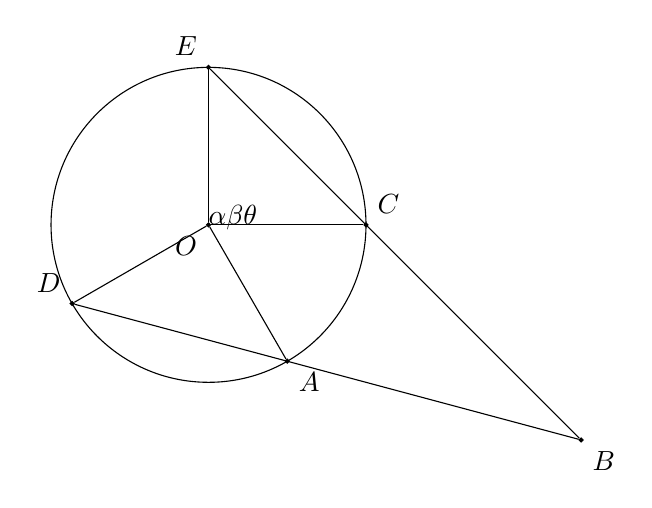
\begin{tikzpicture}
[scale=0.5,>=stealth,point/.style={draw,circle,fill = black,inner sep=0.5pt},]
%\tikzset{shift={(-3,0)}}

%innput parameters
\def\r{4}

%Labeling points
% r sin(pi/3) = 3.4641
\node (O) at (0,0)[point,label=below left:$O$] {};
\node (C) at (\r, 0 )[point,label=above right:$C$] {};
\node (A) at ({\r/2},-3.4641)[point,label=below right:$A$] {};
\node (D) at (-3.4641 , -{\r/2})[point,label=above left:$D$] {};
\node (E) at (0 , \r)[point,label=above left:$E$] {};
\node (B) at (9.4641 , -5.4641)[point,label=below right:$B$] {};


%A



%Drawing parallelogram ABCD
\draw (O) -- (A);
\draw (O) -- (C);
\draw (O) -- (E);
\draw (O) -- (D);
\draw (D) -- (B);
\draw (E) -- (B);
%\draw (C) -- (D);


\draw (O) circle (\r);
%marking angles
\tkzMarkAngle[fill=orange!50,mark=](E,O,D)
\tkzMarkAngle[fill=green!50,mark=](A,O,C)
\tkzLabelAngle[pos=0.65](E,O,D){$\alpha$}
\tkzLabelAngle[pos=0.65](A,O,C){$\beta$}
%\tkzMarkAngle[fill=orange!50,mark=](E,B,D)
\tkzLabelAngle[pos=2.65](E,B,D){$\theta$}

%
\end{tikzpicture}
}
\caption{}
\label{fig:8.5.49_circle}	
\end{figure}
%
\item {\em Construction: }See Fig. \ref{fig:8.5.49_circle}.  The input parameters are
%
\begin{align}
\label{eq:8.5.49_constr_o}
\vec{O} &= \myvec{0\\0} 
\\
\vec{C} &= \myvec{r\\0} 
\label{eq:8.5.49_constr_c}
\end{align}
Then, 
%
\begin{align}
\label{eq:8.5.49_constr_a}
\vec{A} &= r\myvec{\cos \beta \\ -\sin \beta} 
\end{align}

\subitem Equal chords subtend equal angles at the centre.  Hence 
\begin{align}
\phase{EOC} &= \phase{AOD} = \frac{360 \degree - \alpha -\beta}{2}
\\
&= 180\degree - \frac{\alpha+\beta}{2}
\end{align}
Thus, 
\begin{align}
\vec{D} &= r\myvec{\cos \brak{180^{\circ}-\frac{\alpha+\beta}{2}+\alpha} \\ \sin \brak{180^{\circ}-\frac{\alpha+\beta}{2}+\alpha}} 
\\
 &= r\myvec{-\cos \frac{\alpha-\beta}{2} \\ -\sin \frac{\alpha-\beta}{2}}
\label{eq:8.5.49_constr_d}
\\
\vec{E} &= r\myvec{\cos \brak{180^{\circ}-\frac{\alpha+\beta}{2}} \\ \sin \brak{180^{\circ}-\frac{\alpha+\beta}{2}}}
\\
 &= r\myvec{-\cos \frac{\alpha+\beta}{2} \\ \sin \frac{\alpha+\beta}{2}}
\label{eq:8.5.49_constr_e}
\end{align}
\subitem $\vec{B}$ can be found as the intersection of $AD$ and $CE$.



\chapter{Optimization}

%\section{2010}
%\subsection{12}
%\begin{enumerate}

\item One kind of cake requires 300g of flour and 15g of fat, another kind of cake requires 150g of flour and 30g of fat. Find the maximum number of cakes which can be made from 7.5kg of flour and 600g of fat, assuming that there is no shortage of the other ingredients used in making the cakes. Make it as an LPP and solve it graphically.

\end{enumerate}


\chapter{Algebra}
%\section{chapters}
	\item Prove that $ 2\sin^{-1} \brak{\frac{3}{5}} - \tan^{-1} \brak{\frac{17}{31}} = \frac{\pi}{4}$

	\hfill\brak{12, 2016}\item Solve the equation for $x$: $\cos (\tan^{-1}) = \sin \brak{\cot^{-1} \frac{3}{4}} = \sin \brak{\cot^{-1} \frac{3}{4}}$

	
	\hfill\brak{12, 2016}\item Solve for 
	\begin{align*}
		x: \tan^{-1}(x-1) + \tan^{-1}x + \tan^{-1}(x+1) = \tan^{-1}3x
	\end{align*}

	\hfill\brak{12, 2016}\item Prove that 
	\begin{align*}
	\tan^{-1} \brak{\frac{6x-8x^{3}}{1-12x^{2}}} - \tan^{-1} \brak{\frac{4x}{1-4x^{2}}} = \tan^{-1}2x;
	\end{align*}
	\begin{align*}
		\abs{2x} < \frac{1}{\sqrt{3}}
	\end{align*}

 	\hfill\brak{12, 2016}\item Prove that 
	\begin{align*}
		2\sin^{-1}\brak{\frac{3}{5}}-\tan^{-1}\brak{\frac{17}{31}} = \frac{\pi}{4}
	\end{align*}
	\hfill\brak{12, 2016}\item Solve the equation for x:
	\begin{align*}
	\cos\brak{\tan^{-1}x} = \sin\brak{\cot^{-1}\frac{3}{4}}
	\end{align*}
\hfill\brak{12, 2016}

%\section{2015}

\begin{enumerate}
    \item A man walks a certain distance and rides back in $ 3\frac{3}{4} $ hours; he could ride both ways in $ 2\frac{1}{2} $ hours. How many hours would it take him to walk both ways? \hfill(PRERMO 2015)

    \item Positive integers $a$ and $b$ are such that $ a + b = \frac{a}{b} + \frac{b}{a} $. What is the value of $ a^2 + b^2 $? \hfill(PRERMO 2015)

    \item The equations $ x^2 - 4x + k = 0 $ and $ x^2 + kx - 4 = 0 $, where $k$ is a real number, have exactly one common root. What is the value of $ k $? \hfill(PRERMO 2015)

    \item Let $P(x)$ be a non-zero polynomial with integer coefficients. If $ P(n) $ is divisible by $n$ for each positive integer $n$, what is the value of $P(0)$? \hfill(PRERMO 2015)

    \item Let $a$, $b$, and $c$ be real numbers such that $ a - 7b + 8c = 4 $ and $ 8a + 4b - c = 7 $. What is the value of $ a^2 - b^2 + c^2 $? \hfill(PRERMO 2015)

    \item Let $a$, $b$, and $c$ be such that $a + b + c = 0$ and 
    $
    P = \frac{a^2}{2a^2 + bc} + \frac{b^2}{2b^2 + ca} + \frac{c^2}{2c^2 + ab}
    $
    is defined. What is the value of $P$?\hfill(PRERMO 2015)
    \end{enumerate}

%\section{2014}
\begin{enumerate}
\item If real numbers $a, b, c, d, e$ satisfy a + 1 = b + 2 = c + 3 = d + 4 = e + 5 = a + b + c + d + e + 3, what is the value of $a^2 + b^2 + c^2 + d^2 + e^2$?\hfill(PRERMO 2014)
\end{enumerate}

%\section{chapters}
\begin{enumerate}
\item For how many pairs of positive integers \brak{x, y} is x + 3y = 1007\hfill(PRERMO 2012)
\item Rama was asked by her teacher to subtract 3 from a certain number and then divide the result by 9. Instead, she subtracted 9 and then divided the result by 3. She got 43 as the answer. What would have been her answer if she had solved the problem correctly?\hfill(PRERMO 2012)
\item The letters $R$, $M$, and $O$ represent whole numbers. If $R \times M \times O = 240$, $R \times O + M = 46$, and $R + M \times O = 64$, what is the value of $R + M + O$?\hfill(PRERMO 2012)
\item Let $P$\brak{n} = \brak{n + 1}\brak{n + 3}\brak{n + 5}\brak{n + 7}\brak{n + 9} What is the largest integer that is a divisor of $P$(n) for all positive even integers n?\hfill(PRERMO 2012)
\item How many integer pairs \brak{x, y} satisfy $ x ^ 2 + 4y ^ 2 - 2xy - 2x - 4y - 8 =0 $?\hfill(PRERMO 2012)
\item Let $S_n = n^2 + 20n + 12$, $n$ a positive integer. What is the sum of all possible values of $n$ for which $S_n$ is a perfect square?\hfill(PRERMO 2012)
\item Suppose that $4^{x_1} = 5$, $5^{x_2} = 6$, $6^{x_3} = 7, \ldots, 126^{x_{123}} = 127$, $127^{x_{124}} = 128$. What is the value of the product $x_1 x_2 \ldots x_{124}$?\hfill(PRERMO 2012)
\item If
	$\frac{1}{\sqrt{2011} + \sqrt{2012}} = \frac{\sqrt{m} - \sqrt{n}}{\sqrt{m+n}},$
where $m$ and $n$ are positive integers, what is the value of $m + n$?\hfill(PRERMO 2012)
\item If $a = b - c$, $b = c - d$, $c = d - a$, and $abcd \neq 0$, then what is the value of $\frac{a}{b} + \frac{b}{c} + \frac{c}{d} + \frac{d}{a}$? \hfill(PRERMO 2012)
\item How many non-negative integral values of $x$ satisfy the equation
	\begin{align}
    \sbrak{\frac{x}{5}} = \sbrak{\frac{x}{7}}?
	\end{align}
    (Here $\sbrak{x}$ denotes the greatest integer less than or equal to $x$. For example, $\sbrak{3.4} = 3$ and $\sbrak{-2.3} = -3$.)\hfill(PRERMO 2012)
\item Let $x_1, x_2, x_3$ be the roots of the equation $x^3 + 3x + 5 = 0$. What is the value of the expression $ \brak{ x_1 + \frac{1}{x_1} } \brak{ x_2 + \frac{1}{x_2} }\brak{ x_3 + \frac{1}{x_3}}? $\hfill(PRERMO 2012)
\item What is the sum of the squares of the roots of the equation
	\begin{align}
	x^2 - 7\sbrak {x} + 5 = 0?
\end{align}
Here $\sbrak{x}$ denotes the greatest integer less than or equal to $x$. For example, $\sbrak {3.4} = 3$ and $\sbrak{ -2.3} = -3$.\hfill(PRERMO 2012)
\end{enumerate}

%\section{2010}
%\subsection{12}
%	\item Prove that $ 2\sin^{-1} \brak{\frac{3}{5}} - \tan^{-1} \brak{\frac{17}{31}} = \frac{\pi}{4}$

	\hfill\brak{12, 2016}\item Solve the equation for $x$: $\cos (\tan^{-1}) = \sin \brak{\cot^{-1} \frac{3}{4}} = \sin \brak{\cot^{-1} \frac{3}{4}}$

	
	\hfill\brak{12, 2016}\item Solve for 
	\begin{align*}
		x: \tan^{-1}(x-1) + \tan^{-1}x + \tan^{-1}(x+1) = \tan^{-1}3x
	\end{align*}

	\hfill\brak{12, 2016}\item Prove that 
	\begin{align*}
	\tan^{-1} \brak{\frac{6x-8x^{3}}{1-12x^{2}}} - \tan^{-1} \brak{\frac{4x}{1-4x^{2}}} = \tan^{-1}2x;
	\end{align*}
	\begin{align*}
		\abs{2x} < \frac{1}{\sqrt{3}}
	\end{align*}

 	\hfill\brak{12, 2016}\item Prove that 
	\begin{align*}
		2\sin^{-1}\brak{\frac{3}{5}}-\tan^{-1}\brak{\frac{17}{31}} = \frac{\pi}{4}
	\end{align*}
	\hfill\brak{12, 2016}\item Solve the equation for x:
	\begin{align*}
	\cos\brak{\tan^{-1}x} = \sin\brak{\cot^{-1}\frac{3}{4}}
	\end{align*}
\hfill\brak{12, 2016}


\chapter{Geometry}
%\section{chapters}
%\subsection{10}
\begin{enumerate}

\item Write the distance of the following plane from the origin:
    \begin{align*}
    2x - y + 2z + 1 = 0
    \end{align*}

\item Find the points on the line $\frac{x+2}{3} = \frac{y+1}{2} = \frac{z-3}{2}$ at a distance of 5 units from the point $P\brak{1, 3, 3}$.

\item Find the distance of the point $P\brak{6, 5, 9}$ from the plane determined by the points $A\brak{3, -1, 2}$, $B\brak{5, 2, 4}$ and $C\brak{-1, -1, 6}$.

\item Find the coordinates of the foot of the perpendicular and the perpendicular distance of the point $P\brak{3, 2, 1}$ from the plane $2x - y + z + 1 = 0$. Find also, the image of the point in the plane.

\item Find the area of the circle $4x^2 + 4y^2 = 9$ which is interior to the parabola $x^2 = 4y$.

\item Using integration, find the area of the triangle ABD, coordinates of whose vertices are A(4, 1), B(6, 6) and C(8, 4).

\item If the length of three sides of a trapezium other than the base is 10cm each, find the area of the trapezium, when it is maximum.

\end{enumerate}

%\section{2015}
\begin{enumerate}
\item The figure below shows a broken piece of a circular plate made of glass.
    
	  
		\begin{figure}[h!]
    \centering
	    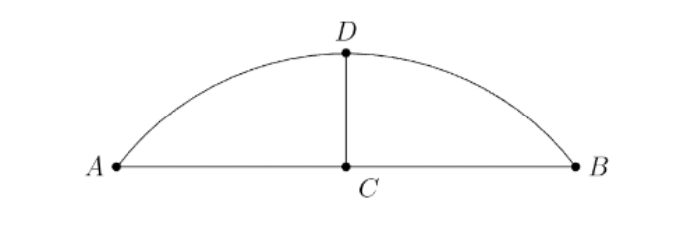
\includegraphics[width=\columnwidth]{olympiad/figs/permo.jpg}
    \end{figure}



    $ C $ is the midpoint of $ AB $, and $ D $ is the midpoint of arc $ AB $. Given that $ AB = 24 $ cm and $ CD = 6 $ cm, what is the radius of the plate in centimeters? (The figure is not drawn to scale.)\hfill(PRERMO 2015)

    \item A $ 2 \times 3 $ rectangle and a $ 3 \times 4 $ rectangle are contained within a square without overlapping at any interior point, and the sides of the square are parallel to the sides of the two given rectangles. What is the smallest possible area of the square? \hfill(PRERMO 2015)

    \item What is the greatest possible perimeter of a right-angled triangle with integer side lengths if one of the sides has length 12? \hfill(PRERMO 2015)

    \item In rectangle $ ABCD $, $ AB = 8 $ and $ BC = 20 $. Let $ P $ be a point on $ AD $ such that $ \angle BPC = 90\degree $. If $ r_1, r_2, r_3 $ are the radii of the incircles of triangles $ APB, BPC $, and $ CPD $, what is the value of $ r_1 + r_2 + r_3 $? \hfill(PRERMO 2015)


\item In the acute-angled triangle $ABC$, let $D$ be the foot of the altitude from $A$, and $E$ be the midpoint of $BC$. Let $F$ be the midpoint of $AC$. Suppose $ \angle BAE = 40\degree $. If $ \angle DAE = \angle DFE $, what is the magnitude of $ \angle ADF $ in degrees?\hfill(PRERMO 2015)

\item The circle $ \omega $ touches the circle $ \Omega $ internally at $ P $. The center $ O $ of $ \Omega $ is outside $ \omega $. Let $XY$ be a diameter of $ \Omega $ which is also tangent to $ \omega $. Assume $ PY > PX $. Let $ PY $ intersect $ \omega $ at $ Z $. If $ YZ = 2PZ $, what is the magnitude of $ \angle LPYX $ in degrees? \hfill(PRERMO 2015)
\end{enumerate}

%\section{2014}
\begin{enumerate}
\end{enumerate}

%\section{chapters}
\begin{enumerate}
\end{enumerate}



\chapter{Discrete}
%\section{2010}
%\subsection{12}
%\begin{enumerate}
\item If the $n^{th}$ term of an $A.P$ is $\brak{2n+1}$, then sum of its first three terms is 
\begin{enumerate}
\item $6n + 3$ 
\item $15$ 
\item $12$ 
\item $21$ 
\end{enumerate}
\item The next terms of $A.P.$ $\sqrt {18}, \sqrt {50}, \sqrt {98}, \ldots$ is 
\begin{enumerate}
\item $\sqrt {146}$ 
\item $\sqrt {128}$ 
\item $\sqrt {162}$ 
\item $\sqrt {200}$ 
\end{enumerate}
%discrete
\item Find the common difference of an $A.P$ whose first term is $5$ and the sum of its first four terms is half the sum of the next four terms. 
%discrete
\item The $17th$ term of an $AP$ is $5$ more than twice its $8th$ term. If the $11th$ term of the $AP$ is $43$, then find the $nth$ term. 

\item Sum of the first $14$ terms of an $AP$ is $1505$ and its first term is $10$. find its $25th$ term. 
\item In an $A.P.$, the first term is $12$ and the common difference is $6$. If the last term of the $A.P.$ is $252$, find its middle term. 
\item If $4$ times the fourth term of an $A.P.$ is equal to $18$ times its $18^{th}$ term, then find its $22^{th}$ term. 
\item The sum of $4^{th}$ and $8^{th}$ term terms of an $A.P.$ is $24$ and the sum of its $6^{th}$ and $10^{th}$ terms is $44$. Find the sum of first ten terms of the $A.P.$ 
\end{enumerate}

%\section{2014}
\begin{enumerate}
	\item What is the number of ordered pairs $\brak{A, B}$ where $A$ and $B$ are subsets of $\{1, 2, \ldots, 5\}$ such that neither $A \subseteq B$ nor $B \subseteq A$?\hfill(PRERMO 2014)
	\item
The Bank of Oslo issues two types of coin: aluminium \brak{denoted \ A} and bronze \brak{denoted \ B}. Marianne has $n$ aluminium coins and $n$ bronze coins, arranged in a row in some arbitrary initial order. A chain is any subsequence of consecutive coins of the same type. Given a fixed positive integer $k$ $\leq$ $2n$, Marianne repeatedly performs the following operation: she identifies the longest chain containing the $k^{th}$  coin from the left, and movees all coins in that chain to the left end of the row. For example, if $n = 4$ and $k = 4$, the process starting from the ordering $AABBBABA$
 would be 
\begin{align}
A A \underline{B} B B A B A \rightarrow B B B \underline{A} A A B A \rightarrow A A \underline{A} B B B B A \rightarrow B B B \underline{B} A A A A \rightarrow .... 
\end{align}
Find all pairs \brak{n,k} with $\brak{1 \leq k \leq 2n }$ such that for every initial ordering, at some moment during the process, the leftmost \brak {n} coins will all be of the same type. 
\hfill(IMO 2022)
\item
Let  $n$ be a positive integer. A Nordic square is an  $n \times n$ board containing all the integers from  $1$ to  $n^{2}$ so that each cell contains exactly one number. Two different cells are considered adjacent if they share a common side. Every cell that is adjacent only to cells containing la
Rger numbers is called a valley. An uphill path is a sequence of one or more cells such that:
\begin{enumerate}
\item
The first cell in the sequence is a valley,
\item
Each subsequent cell in the sequence is adjacent to the previous cell, and
\item
The numbers written in the cells in the sequence are in increasing order.
\end{enumerate}
Find as a function of  $n$, the smallest possible total number of uphill paths in a Nordic square. \hfill(IMO 2022)
\item
Let  $n$  be a positive integer. A $Japanese \ triangle$ consists of  $1 + 2 + \cdots + n$  circles arranged in an equilateral triangular shape such that for each  $i = 1, 2, \ldots, n$  the  $i^{th}$ row contains exactly  $i$  circles, exactly one of which is coloured red. A ninja path in a $Japa
nese \ triangle$ is a sequence of  $n$  circles obtained by starting in the top row, then repeatedly going from a circle to one of the two circles immediately below it and finishing in the bottom row. Here is an example of a $Japanese \ triangle$ with $ n = 6$  along with a $ninja \ path$ in that tr
iangle containing two red circles.
\begin{figure}[h!]
\centering
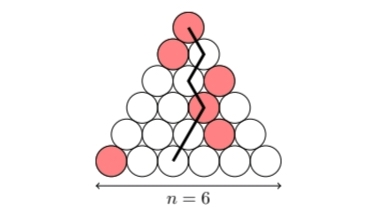
\includegraphics[width=\columnwidth]{figs/img1.jpg}
\caption{Image 1}
\end{figure}
In terms of  $n$, find the greatest $k$ such that in each $Japanese \ triangle$ there is a $ninja \ path$ containing at least  $k$ red circles. \hfill(IMO 2023)
\item
Determine all pairs  $\brak{a, b}$  of positive integers for which there exist positive integers  $g$ and $N$ 
Such that \begin{align}
gcd \brak{a^{n} + b, b + a} = g
\end{align}
Holds for all integers $n \geq N$. Note that $\gcd\brak{x, y}$ denotes the greatest common divisor of integers $x$ and $y$. \hfill(IMO 2024)
\item
Let  $a_{1}, a_{2}, a_{3}, \ldots$  be an infinite sequence of positive integers, and let $N$  be a positive integer. Suppose that, for each  $n \ge N$ ,  $an$ is equal to the number of times  $an$ appears in the list  $a_{1}, a_{2}, \ldots, a_{n-1}$. 
\\ Prove that at least one of the sequences $ a_{1}, a_{3}, a_{5}, \ldots $ and $ a_{2}, a_{4}, a_{6}, \ldots $ is eventually periodic.
		An infinite sequence $b_{1}, b_{2} b_{3}, \ldots$ is eventually periodic if there exist positive integers  $p$  and   $M$ such that  $b_{m+p} = b_{m}$  for all  $m \geq M$ . \hfill(IMO 2024)	
\item
Turbo the snail plays a game on a board with  $2024$ rows and  $2023$  columns. There  are hidden monsters in $2022$ of the cells. Initially, Turbo does not know where any of the monsters   are, but he knows that there Is exactly one monster in each row except the first row and the last  row, and 
That each column contains at most one monster.
Turbo makes a series of attempts to go from the first row to the last row. On each attempt, he chooses   to start on any cell in the first row, then repeatedly moves to an adjacent cell sharing a common Turbo the Tortoise is on a quest to escape from a rectangular grid of cells. Starting on any ce
Ll in the first row, Turbo repeatedly moves to an adjacent cell sharing a common side.\brak{\text{He is allowed to return to a previously }} If he reaches a cell with a monster, his attempt ends and he is transported back to the first row to start a new attempt. The monsters do not move, and Turbo r
emembers whether or not each cell he has visited contains a monster. If he reaches any cell in the last row, his attempt ends and the game is over.
Determine the minimum value of $ n $ for which Turbo has a strategy that guarantees reaching the last row on the  $n^{th}$ attempt or earlier, regardless of the locations of the monsters. \hfill(IMO 2024) 
\item Let
$ S_n = \sum_{k=0}^{n} \frac{1}{\sqrt{k+1} + \sqrt{k}}. $
What is the value of 
$ \sum_{n=1}^{90} \frac{1}{S_n + S_{n-1}}? $\hfill(Prermo 2013)

\item An infinite sequence $x_0, x_1, x_2,.... $of real numbers is said to be bounded if there is a constant $C$ such that $\mydet{x_i} \leq C$ for every $i \geq 0$.
	  Given any real number $a > 1$, construct a bounded infinite sequence $x_0, x_1, x_2,.....$ Such that
	  \begin{align*}\mydet{x_i-x_j}\mydet{i-j}^a \geq 1 \end{align*}
	  for every pair of distinct nonnegative integers $i, j$.\hfill(IMO 1991)
	  \item  Let $n$ be a fixed integer, with $n \geq 2$.$\brak{a}$ Determine the least constant $C$ such that the inequality \begin{align*}\sum_{1\leq i<j\leq n} {x_{i}} {x_{j}} \brak{x_{i}^2 + x_{j}^2} \leq C \brak{\sum_{1\leq i\leq n} x_{i}}^4\end{align*} holds for all real numbers ${x_{1}},....,{x_{n}} \geq 0$. $\brak{b}$ For this constant $C$, determine when equality holds.\hfill(IMO 1999) 

\item  $A$,$ B$, $C$ are positive reals with product$1$. Prove that $\brak{A-1+\frac{1}{B}}\brak{B-1+\frac{1}{C}}\brak{C-1+\frac{1}{A}} \leq 1$.\hfill(IMO 2000)

\item Determine all positive integers relatively prime to all the terms of the infinite sequence
 \begin{align*}
 a_n={2^n}+{3^n}+{6^n},n\geq{1}.
\end{align*} \hfill(IMO 2005)
\item In a mathematical compentition some competitors are friends. Friendship is always mutual. Call a group of competitors a clique if each two of tem are friends.(In particular, any group of fewer than two competitors is a clique.) The number of members of a clique is called its size.                                    Given that, in this competition, the largest size of a clique is even, prove that the competitors can  be arranged in two rooms such that the largest size of  a clique contained in one room is the same as the largest size of a clique contained in the other room.\hfill(IMO 2007)
		\item  Let $n$ and $k$ be positive integers with $k\geq n$ and $k-n$ an even number. Let $2n$ lamps labelled $1, 2,\dots, 2n$ be given, each of which can be either on or off. Initially all the lamps are off.We consider sequences of steps: at each step one of the lamps is switched ( from on to off or from off to on).                                                       Let $N$ be the number of such sequences consisting of $    k$ steps and resulting in the state where lamps $1$ thr    ough $n$ are all on, and lamps $n + 1$ through $2n$ are     all off.                                         Let $M$ be the number of such sequences consisting of $k$ steps, resulting in the state where lamps $1$ through $n$ are all on, and lamps $n + 1$ through $2n$ are all off, but where none of the lamps $n + 1$ through $2n$ is ever switched on.  
		\item Find all functions $f$ : $\brak {0,\infty}$ $\rightarrow$ $\brak{0}$, $\infty$  so, (f is a function from the positive real numbers to the positive real numbers) such that $\frac{(f(w))^2 + (f(x))^2} {f(y)^2 + f(z)^2 }$  for all positive real numbers $w, x, y,z$, satisfying $wx$ = $yz$.\hfill(IMO 2008)
	\item Let $n$ be a positive integer $a_{1},\dots,a_{k}\brak{k\geq 2}$ be distinct integer in the set $\cbrak{1 ,\dots, n}$ such that $n$ divides $a_{i} \brak{a_{i+1}-1}$ for $i=1,\dots, k-1$. Prove that $n$ does not divide $ a_{k} \brak {a_{i}-1}$.\hfill(IMO 2009)
	\item Suppose that $s_{1}, s_{2}, s_{3},\dots $ is a strictly increasing sequence of positive integers such th    at the subsequences       
		\begin{align}
			s_{s1}, s_{s2}, s_{s3},\dots and s_{s1+1}, s_{s2+1}, s_{s3+1},\dots
       \end{align}
are both arithmetic progressions. Prove that the sequence $s_1,s_2,s_3$,...is itself an arithmetic progession.\hfill(IMO 2009) Determine the ratio $\frac{N}{M}$.\hfill(IMO 2008)
\item Find all integers $n\leq3$ for which there exist real numbers \begin{align}01.02.02,\end{align} such that \begin{align} an+1=a1   and  an+2=a2,and \end{align} \begin{align}i=1,2,...,n. aiai+1+1=ai+2 for i=1,2,.....n\end{align}.\hfill (IMO 2018)
\item $A$ site is any point $(x,y)$ in the plane such that $z$ and $y$ are both positive integers less than or equal to $20$.Initially, each of the $400$ sites is unoccupied. Amy and Been take turns placing stones with Amy going first. On her turn, Amy places a new red stone on an unoccupied site such that the distance between any two sites occupied by red stones is not equal to $sqrt(5)$ On his turn, Ben places a new blue stone on any unoccupied site.
	(A site occupied by a blue stone is allowed to be at any distance from any other occupied site.) They stop as soon as a player cannot place a stone. Find the greatest $K$ such that Amy can  ensure that she places at least $K$ red stones, no matter how Ben places his blue stones. \hfill (IMO 2018)
	\item Show that there exists a set $A$ of positive  integers with the following property: For any infinite set {S} of primes there exist two positive integers $m$ $\epsilon$ $A$ and $n \notin A$ each of which is a product of $k$ distinct elements of $S$ for some $k \geq 2$.   \hfill(IMO 1994)
\end{enumerate}


\chapter{Number Systems}
%\section{chapters}
%\subsection{12}
\begin{enumerate}
    \item Let $n$ be a positive integer such that $1 \leq n \leq 1000$. Let $M_n$ be the number of integers in the set 
	    $X_n =  \cbrak{ \sqrt{4n+1}, \sqrt{4n+2}, \ldots, \sqrt{4n+1000} }$.
		Let 
		\begin{align}
a = \max{M_n : 1 \leq n \leq 1000},
		\end{align}
	and	\begin{align}
b = \min{M_n : 1 \leq n \leq 1000}.		
		\end{align}
		\\Find $a - b$.\hfill(IOQM 2015)
    
    \item Find the number of elements in the set
	    \begin{align}
   \brak{a, b} \in \cbrak{N} : 2 \leq a, b \leq 2023, \log_a \brak{b} + 6 \log_b \brak{a} = 5.
	    \end{align}\hfill(IOQM 2015)


    \item Let $\alpha$ and $\beta$ be positive integers such that 

	    \begin{align}
\frac{16}{37} < \frac{\alpha}{\beta} < \frac{7}{16}.
	    \end{align}
 Find the smallest possible value of $\beta$.\hfill(IOQM 2015)
    
    \item For $n \in N$ , let $P\brak{n}$ denote the product of the digits in $n$ and $S\brak{n}$ denote the sum of the digits in $n$ . Consider the set 
	    \begin {align}
		A =  \cbrak{ n \in N : P\brak{n}  is  non-zero, square  free  and  S\brak{n}  is  a  proper  divisor   of   P\brak{n} }.
		\end {align}
Find the maximum possible number of digits of the numbers in $A$ .\hfill(IOQM 2015)
    
    \item For any finite non-empty set $X$ of integers, let $\max\brak{X}$ denote the largest element of $X$ and $|X|$ denote the number of elements in $X$. If $N$ is the number of ordered pairs $\brak{A, B}$ of finite non-empty sets of positive integers, such that
	    \begin{align}
\max(A) \times |B| = 12 \quad \text{and}
	    \end{align}
		\begin{align}
			\quad |A| \times \max\brak{B} = 11,
		\end{align}
 and $N$ can be written as $100a + b$ where $a, b$ are positive integers less than 100, find $a + b$.\hfill(IOQM 2015)
 \item The sequence $\langle a_n \rangle_{n \geq 0}$ is defined by $a_0 = 1$, $a_1 = -4$, and $a_{n+2} = -4a_{n+1} - 7a_n$ for $n \geq 0$. Find the number of positive integer divisors of $a_{250} - a_{49} a_{51}$.\hfill(IOQM 2015)
    
    \item A quadruple $\brak{a, b, c, d}$ of distinct integers is said to be balanced if $a +b = c + d$ and $a < b < c < d$. Find the number of balanced quadruples of distinct integers in the set $\cbrak{1, 2, \cdots, 12}$.\hfill(IOQM 2015)
     \item There is an integer $n>1$. There are n2 stations on a slope of a mountain, all at
different altitudes. Each of two cable car companies, A and B, operates k cable cars; each cable
car provides a transfer from one of the stations to a higher one (with no intermediate stops). The
k cable cars of A have k different starting points and k different finishing points, and a cable car
which starts higher also finishes higher. The same conditions hold for B. We say that two stations
are linked by a company if one can star using
one or more cars of that company (no other movements between stations are allowed).
Determine the smallest positit from the lower station and reach the higher one byve integer k for which one can guarantee that there are two stations
that are linked by both companies.
\hfill(IMO 2020)
\item Find the smallest positive integer $ k $ such that 
$ k(3^3 + 4^3 + 5^3) = a^n $ for some positive integers $ a $ and $ n $, with $ n > 17 $.\hfill(Prermo 2013)

\item Let $ S(M) $ denote the sum of the digits of a positive integer $ M $ written in base 10. Let $ N $ be the smallest positive integer such that $ S(N) = 2013 $. What is the value of $ S(5N + 2013) $?\hfill(Prermo 2013)

\item Let $ m $ be the smallest odd positive integer for which
$ 1 + 2 + \cdots + m $
is a square of an integer and let $ n $ be the smallest even positive integer for which
$ 1 + 2 + \cdots + n $
is a square of an integer. What is the value of $ m + n $?\hfill(Prermo 2013)

\item What is the maximum possible value of $ k $ for which 2013 can be written as a sum of $ k $ consecutive positive integers?\hfill(Prermo 2013)
\item Let $a,b$ and $c$ be positive integers, no two of which have a common divisor grater than $1$. Show that $2abc-ab-bc-ca$ is the largest integer which cannot be expressed in the form $xbc+yca+zab$, where $x,y$ and $z$ are non-negative integers.\hfill(IMO 1983)

\item Is it possible to choose $1983$ distinct positive integers, all less than or equal to $10^5$, no three of which are consecutive terms of
an arithmetic progression ? justify your answer.\hfill(IMO 1983)

\item Find one pair of positive integers $a$ and $b$ such that :
	$\brak{i}$ $ab\brak{a+b}$ is not divisible by $7$;
	$\brak{ii}$$\brak{a+b}^7-a^7-b^7$ is divisible by $7^7$\hfill(IMO 1984)


\item Let $a,b,c$ and $d$ be odd integers such that  $0<a<b<c<d$ and $ad=bc$. Prove that if $a+d=2^k$ and $b+c=2^m$ for some integers $k$ and   $m$, then $a=1$\hfill(IMO 1984)

\item Let  $n$ and $k$ be given relatively prime natural numbers $k<n$.Each number in the set $M={1,2,...n-1}$ is colored either blue or white. It is given that
	$\brak{i}$ for each $i  \epsilon   M$, both $i$ and $n-i$ have the same color;
	$\brak{ii}$ for each $i \epsilon  M$, $i\neq k$, both $i$ and $\mydet{i-k}$ have the same color. Prove that all numbers in $M$ must have the same color.\hfill(IMO 1985)

\item Given a set $M$ of $1985$ distinct positive integers, none of which has a prime divisor grater than $26$. Prove that $M$ contains at least one subset of four distinct elements whose product is the fourth power of an integer.\hfill(IMO 1985)


\item For every real number $x_1$, construct the sequence $x_1, x_2, ..116  . $by setting 
	\begin{align*} x_{n+1}=x_n\brak{x_n+\frac{1}{4}}\end{align*} for each $n \geq 1$ Prove that there exists exactly one value of $x_1$ for which  \begin{align*} 
0 < x_n<x_{n+1}<1 \end{align*} for every $n$.\hfill(IMO 1985)
\item Let $1 \leq r \leq n$ and consider all subsets of $r$ elements of the set $\cbrak{1,2,..., n}$. Each of these subsets has a smallest  member. Let $F\brak{n,r}$ denote the arithmetic mean of these smallest numbers; prove that $F\brak{n,r}= \frac{n+1}{r+1}$ \hfill(IMO 1981)


 \item \brak{a} For which values of $n > 2$ is there a set of $n$ consecutive positive integers such that     the largest number in the set is a divisor of the least common multiple of the remaining $n-1$ numbers
	 \brak{b}For which values of $n > 2$ is there exactly one set having the stated property?\hfill(IMO 1981)
\item . The function $f\brak{n}$ is defined for all positive integers $n$ and takes on non-negative integer values. Also, for all $m,n$
  \begin{align*}f\brak{m + n} - f\brak{m} - f\brak{n} = 0  \brak{or} 1 \end{align*}
 \begin{align*}f\brak{2} = 0  , f\brak{3} > 0,and  f\brak{9999} = 3333.\end{align*}
       Determine $f\brak{1982}.$ \hfill(IMO 1982)
\item Prove that if $n$ is a positive integer such that the equation. \begin{align*}x^3 - 3xy^2 + y^3 =
n \end{align*}  has a solution in integers $\brak{x, y}$, then it has at least three such solutions. Sh
w that the equation has no solutions in integers when $n = 2891.$ \hfill(IMO 1982)
	\item Consider the infinite sequences $\cbrak{x_n}$ of positive real numbers with following properties:     
             $ x_{0}=1,$ and for  all  $i \geq 0, x_{i+1} \leq x_i.$ 
 \brak{a} Prove that for every such sequence, there is $n \geq 1$ such that
                      \begin{align*} \frac{x^{2}_{0}}{x_{1}}+ \frac{x^{2}_{1}}{x_{2}}+ ...+\frac{x^{2}_{n- 1}}{x_{n}} \geq 3.999.\end{align*}
 \brak{b} Find such a sequence for which
                    \begin{align*} \frac{x^{2}_{0}}{x_{1}}+ \frac{x^{2}_{1}}{x_{2}}+ ...+\frac{x^{2        }_{n1}}{x_{n}}< 4.\end{align*} \hfill(IMO 1982)
                    \item  Let $d$ be any positive integer not equal to $2$, $5$, or $13$. Show that one can find distinct $a$, $b$ in the set $\cbrak{2, 5, 13. d}$ such that $ab-1$ is not a perfect square.\hfill(IMO 1986)

\item Let $p_n \brak{k}$ be the number of permutations of the set $\cbrak{1,\dots
	    ,n}$, $n\geq1$,which have exactly $k$ fixed points.Prove that 
		                 \begin{align*}   \sum_{k=0}^{n} k \cdot p_n\brak{k} = n
					             \end{align*}
(Remark:A permtation $f$ of a set $S$ is one-to-one mapping of $S$ onto itself.An element $i$ in $S$ is called a fixed point of the the permutation $f$ if f\brak{i}=i. ) \hfill(IMO 1987)

\item Let $n$ be a positive integer and let $A_1, A_2, \dots, A_{2n+1}$ be subsets o
    f a set $B$. Suppose that 
                 $\brak{a}$ Each $A_i$ has exactly $2n$ elements,
                  $\brak{b}$ Each $A_i \cap A_j \brak{1\leq i \leq j\leq 2n+1}$contains exactl
    y one element, and \\
                  $\brak{c}$ Every element of $B$ belongs to at least two of the $A_i$.
                  
                 For which values of $n$ can one assign to every element of $B$ one of the numbers $0$ and $1$ in such a way that $A_i$ has $0$ assigned to exactly $n$ of its elements?\hfill(IMO 1988)
\item Let $a$ and $b$ be positive integers such that $ab + 1$ divides $a^2 + b^2$. Show that 
               \begin{align*} \frac{a^2+b^2}{ab+1} \end{align*} is the square of an integer.\hfill(IMO 1988)
               \item problem 1 Prove that for any pair of positive integers $k$ and $n$, there exist $k$ positive integers $m_1,m_2,m_3,\ldots$
 (not necessarily different) such that
\begin{align}
	1+\frac{2^{k}-1}{n}=\brak{1+\frac{1}{m_1}}\brak{1+\frac{1}{m_2}}\ldots\brak{1+\frac{1}{m_k}}
\end{align}  \hfill(Imo 2013)
 \item problem2 let $a_{0<} a_{1<} a_{2 <} \ldots$ be an infinite sequence of positive integers.prove that there exists a unique integer $n    \geq 1$such that          \begin{align}                                                                                                                                                                             a_{n< }\frac{a_0+a1+\ldots+a_n}{n} < a_{n+1}.                                                                                                                \end{align} \hfill(Imo2014) \hfill(Imo 2014)   
\item Problem 3. For each positive integer $n,$ the Bank of Cape Town ienes coins of denomination$\frac{1}{n}$ Given a finite collection of such coins (of  not  necessarily  differ
    ent  denominations) with total value at most $99 +\frac{1}{2}$ prove that it is possible to split this collection into $100$ or fewer groups, such that each group has total value at most $1$. \hfill(Imo2014)
    \item Prove that for each positive integer $n$ there exist $n$ consecutive positive integers none of which is an integral power of a prime number. \hfill(IMO 1989)

	\item A permutation $\brak{x_1,x_2,....,x_m}$ of the set \{1,2.....,2n\}. where $a$ is a positive integer, is said to have property $P$ if $\mydet{x_i - x_{i+1}} = n $ for at least one in\{1,2,....,2n-1\}. Show that, for each $n$, there are more permitations with property $P$ than without.\hfill(IMO 1989)

	\item Determine all integers $n>1$  such that
		\begin{align*} \frac{{2^n}+1}{n^2}\end{align*}is integer.\hfill(IMO 1990)


 \item Given a triangle $ABC$, let $I$ be the center of its inscribed circle. The internal bisectors of the angles $A, B, C$ meet the opposite sides in $A', B', C'$ respectively. Prove that
	 \begin{align*}\frac{1}{4} < \frac{AI. BI. CI.}{AA'. BB'. CC'.}\leq\frac{8}{27}\end{align*}. \hfill(IMO 1991)


\item Let $n > 6$ be an integer and $a_1, a_2,....,a_k $ be all the natura numbers less than $n$ and relatively prime to $n$ If \begin{align*}
a_2-a_1=a_3-a_2=......=a_k-a_{k-1} > 0,\end{align*}
       prove that $n$ must be either a prime number or a power of 2.\hfill(IMO 1991)
       \item In a finite sequence of real numbers the sum of any seven successive terms is negative, and the sum of any eleven successive terms is positive. Determine the maximum number of terms in the sequence.\hfill(Imo 1977)

\item 	Let $n$ be a given integer > $2$, and let $V_{n}$ be the set of integers $1+ kn$, where $k = 1, 2 ,\ldots A$ number $m \epsilon V_{n}$ is called indecomposable in $V_{n}$, if there do not exist numbers $p$ ,$q \epsilon V_{n}$ such that $pq = m$. Prove that there exists a number $r \epsilon V_{n}$ that can be expressed as the product of elements indecomposable in $V_{n}$ in more than one way. (products which differ only in the order of their factors will be considered the same).\hfill(Imo 1977)

\item Let $a$ and $b$ be positive integers. When $a^2 + b^2$ is divided by $a+b$, the quotient is $q$ and the remainder is $r$. Find all pairs \brak{a, b} such that $q^2 + r = 1977.$ \hfill(Imo 1977)

\item	Let $f\brak{n}$ be a function defined on the set of all positive integers and having all its values in the same set. Prove that if \begin{align}f\brak{n + 1} > f\brak{f\brak{n}}\end{align} for each positive integer $n$, then \begin{align}f\brak{n} = n\end{align} for each $n$
		\hfill(Imo 1977)

	\item $m$ and $n$ are natural numbers with $1 \leq m \textless n$ In their decimal representations, the last three digits of $1978$ are equal, respectively, to the last three digits of $1978$". Find $m$ and $n$ such that $m+n$ has its least value.\hfill(Imo 1978)

\item The set of all positive integers is the union of two disjoint subsets 
\begin{align}
{f\brak{1}, f\brak{2} ,\ldots,f\brak{n},\ldots} ,{ g\brak{1},g\brak{2},\ldots,g\brak{n},\ldots} 
\end{align},where
\begin{align}
f\brak{1}< f\brak{2} < \ldots < f\brak{n} < \ldots,\\ g\brak{1} < g\brak{2} < \ldots < g\brak{n}< \ldots\\, and,   g\brak{n}=f\brak{f\brak{n}} + 1
\end{align}
for all $n \geq 1$ and Determine $ƒ\brak{240}.$\hfill(Imo 1978)

\item Let ${a_{k}\brak{k=1,2,3.\ldots,n,\ldots}}$ be a sequece of distinct positive integers. Prove that for all natural numbers $n$,\begin{align}\sum_{k=1}^{n} \frac{a_{k}}{k^2} \geq \sum_{k=1}^{n} \frac{1}{k}\end{align}\hfill(Imo 1978)

\item Let $p$ and $q$ be natural numbers such that \begin{align}\frac{p}{q}=-\frac{1}{2}+\frac{1}{3}-\frac{1}{4}+\ldots -\frac{1}{1318}+\frac{1}{1319}\end{align}.Prove that $p$ is divisible by $1979$.\hfill(Imo 1979)

\item For any positive integer $n$, let d{\brak{n}} denote the number of positive divisors of $n$ (including $1$ and $n$ itself). Determine all positive integers k such that $ \frac{d\brak{n^2}} {d\brak{n}}  = k$ for some $n$.\hfill(IMO 1998) 

\item Determine all pairs \brak{a, b} of positive integers such that $ab^2 + b + 7$ divides $a^2    b + a + b$.\hfill(IMO 1998)

\item  Consider all functions $f$ from the set $N$ of all positive integers into itself satisfying $f\brak{t^2f\brak{s}} = s\brak{f\brak{t}}^2$ for all $s$ and $t$ in $N$. Determine the least possible value of ${f\brak{1998}}$.\hfill(IMO 1998)

\item Determine all pairs \brak{n,p} of positive integers such that$p$ is a prime,$n$ not exceeded $2p$,and$\brak{p-1}^n+1$ is divisible by $n^{p-1}$.\hfill(IMO 1999)

\item Can we find $N$ divisible by just $2000$ different primes, so that $N$ divides $2^N + 1$? [$N$ may be divisible by a prime power.]\hfill(IMO 2000)    
\item Let $ABC$ be a triangle with incentre I.A point P in the interior of the triangle satisfies
\begin{align*}
\angle{PBA} + \angle{PCA} = \angle{PBC}+ \angle{PCB} \end{align*} 
Show that $AP\geq{AI}$,and that equality holds if only if $P=I$.\hfill(IMO2006)
\item Determine all pairs (x,y) of integers such that
 \begin{align*}
 1+2^{x}+2^{x+1}=y^{2}
 \end{align*}\hfill(IMO 2006)
 \item Let $N$ be the set of positive integers. Determine all functions $g:N \rightarrow N $ such that
				\begin{align}
					(g(m)+n) (m+g(n))
				\end{align}
				is a perfect square for all $m,n \in N $.\hfill(IMO2010)
			\item In each of six boxes $B_{1}, B_{2}, B_{3}, B_{4}, B_{5}, B_{6}$ there is initially one coin. There are two types of operation allowed:
				Type $1$: Choose a nonempty box $B_{j}$ with $1\leq{j}\leq{5}$. Remove one coin from $B_{j}$ and add two coins to $B_{j+1}$.
				Type $2$: Choose a nonempty box $B_{k}$ with $1\leq{k}\leq{4}$. Remove one coin from $B_{k}$ and exchange the contents of (possible empty) boxes $B_{k+1}$ and $B_{k+2}$.
				Determine whether there is a finite sequence of such operations that results in boxes $B_{1}$, $B_{2}$, $B_{3}$, $B_{4}$, $B_{5}$ being empty and box $B_{6}$ containing exactly $2010^{2010^{2010}}$ coins. (Note that $a^{(b^{c})}$.)\hfill(IMO2010)
			\item Let $a_{1}, a_{2}, a_{3}$,\dots be a sequence of positive real numbers. Suppose that for some positive integer $s$, we have
				\begin{align}
					a_{n}=max\{a_{k}+a_{n-k}\vert1\leq{k}\leq{n-1}\}
				\end{align}
				for all $n>s$. Prove that there exist positive integers $l$ and $N$, with $l\leq{s}$ and such that $a_{n}=a_{l}+a_{n-l}$ for all $n\leq{N}$.\hfill(IMO2010)
			\item Given any $setA=\{a_{1}, a_{2}, a_{3}, a_{4}\}$ of four distinct positive integers, we denote the sum $a_{1}+a_{2}+a_{3}+a_{4}$ by $s_{A}$. Let $n_{A}$ denote the number of pairs $ ( i, j) $ with $1\leq{i}\leq{j}\leq{4}$ for which $a_{i}+a_{j}$ divides $s_{A}$. Find all sets $A$ of four distinct positive integers which achieve the largest possible value of $n_{A}$.\hfill(IMO2011)
			\item  Let $f$ be a function from the set of integers to the set of positive integers. Suppose that, for any two integers $m$ and $n$, the difference $f\brak m -f\brak n$ is divisible by $f( m-n)$. Prove that, for all integers $m$ and $n$ with $f \brak m \leq{f\brak n}$, the number $f\brak n$ is divisible by $f\brak m$.\hfill(IMO2011)
			\item  Let $n\geq{3}$ be an integer, and let $a_{2}, a_{3},\dots, a_{n}$  be positive real numbers such that $a_{2}a_{3} \dots a_{n}=1$. Prove that
				\begin{align}
					(1+a_{2}) ^{2}  (1+a_{3}) ^{3} \dots (1+a_{n}) ^{n} > n^{n}.\hfill(IMO2012)
				\end{align}
			\item Find all functions $f:Z \rightarrow Z $ such that, for all integers $a, b, c$ that satisfy $a+b+c = 0$, the following equality holds:
				\begin{align}
					f(a)^2+f(b)^2+f(c)^2=2f(a)f(b)+2f(b)f(c)+2f(c)f(a).
				\end{align}
				(Here $Z$ denotes the set of integers.)\hfill(IMO2012)
				\brak a Prove that, for any real numbers $x_{1} \leq x_{2} \leq \dots \leq x_{n}$ 
	 $\{ | x_{i} - a_{i} | : 1 \leq  i \leq n \} \geq$  $\frac {d}{2}$. \brak *                                \brak b Show that there are real numbers $x_{1} \ leq x_{2} \leq \dots \leq x_{n}$ such that equality holds in \brak *.\hfill(IMO 2007)
\item Let $a and b$ be positive integers. Show that if     $4ab-1$ divides $(4a^2-1)^2$, then $a=b$.\hfill(IMO 2007)
\item Let $n$ be a positive integer. Consider           $S={(x,y,z)} : {x,y,z} \epsilon i{0,1,\dot,n}$,     ${x+y+z>0}$  as a set of $(n+1)^{3}-1$ points in three-dimensional space.Determine the smallest possible number of planes, the union of which contains $S$ but doesnot include $(0,0,0)$.\hfill(IMO 2007) 
	\item Prove that                                         7 $\frac{x^2}{{(x-1)}^{2}}$+$\frac{y^2}{{(y-1)}^{2}}$+$\frac{z^2}{{(z-1)}^{2}} \geq 1$
	for all real numbers $x, y, z$, each different from $1$, and satisfying $xyz = 1$.$\brak
{b}$  Prove that equality holds above for infinitely many triples of rational numbers $x, y, z$, each different from  $1$, and satisfying $xyz=1$.\hfill(IMO 2008)
\item Prove that there exist infinitely many po    sitive integers $n$ such that $n^2+1$ has a prime divis    or which is greater than $2n+\sqrt2n$.\hfill(IMO 2008)

\item  Determine all functions $f$ from the set of positive integers to the set of positive integers such that, for all positive integers $a$ and $b$, there exists a non-degenerate triangle with sides of lengths \\$a, f (b)$ and $f (b+f(a)-1).$ \\
                $(A triangle is non-degenerate if its v    ertices are not collinear)$.\hfill(IMO 2009)
		\item Let $a_{1}$, $a_{2}$,\dots, $a_{n}$ be distinct positive integers and let $M$ be a set of $n-1$ positive integers not containing $s = a_{1}+a_{2}$+ \dots + $a_{n}$. A grasshopper is to jump along the real axis, starting at the point 0and making $n$ jumps to the right with lengths $a_{1}, a_{2}\dots,a_{n}$ in some order. Prove that the order can be chosen in such a way  that the grasshopper never lands on any point in $M$.\hfill(IMO 2009)
		\item Find all positive integers $n$ for which each cell of     an $n\times n$ table can be filled with one of the letters \begin{align}I,M and O\end{align} in such a way that:                                    in each row and each column,one third of the entries are $I$,one third are $M$ and one third are $O;$and in any diagonal,if the number of entries on the diagonal is a multiple of three,the$n$ one third of the entries are $I,$ one thirdv are $M$ and one third are $O.$\hfill (IMO 2016)
\item $A$ set of positive integers is called fragrant if it contains at least two elements and each of its elements has a prime factor in common with at least one of the other elements. Let $P(n) = n ^ 2 + n + 1$ What is the least possible value of the positive integer $b$ such that there exists a  non-negative integer a for which the set \begin{align}{P(a + 1), P(a + 2) ,...,P(a+b)}\end{align} is fragrant?\hfill (IMO 2016)
(a) Prove that Geoff can always fulfil his wish if $n$ is odd.                                       (b) Prove that Geoff can never fulfil his wish if $n$ is even.
\item An ordered pair $(x, y)$ of integers is a primitive point if the greatest common divisor of $r$ and $y$     is $1$. Given a finite set $S$ of primitive points, prove that there exist a positive integer $n$ and integers $ao$, $41$, $4$ such that, for each $(x, y)4$ in $S$, we have\hfill (IMO 2017)                           \begin{align}a_0x^n + a_1x^{n-1}y + a_2x^{n-2}y^2 + \cdots + a_{n-1}xy^{n-1} + a_ny^n = 1.\end{align}
		\item Let $a1,a2$,... be an infinite sequence of positive integers. Suppose that there is an integer $N\>1$ such that, for each $n\neq N$, the number $01$ is an integer. Prove that there is a positive integer $M$ such that for all $m1>=M$.\hfill (IMO 2018)
 \item  Find all integers $a,b,c$ with $1 < a < b <c$ such that  \hfill(IMO 1992)                                        
 $(a-1)(b-1)(c-1)$ is a divisor of $abc$ - $1$.
\item For each positive integer $n$, $S(n)$ is defined to be the greatest integer such that, for every positive integer $k$ $\leq$ $S(n)$, $n^{2}$ can be  written as the sum of $k$ positive squares.  \hfill(IMO 1992)       

$(a)$ Prove that $S(n)$ $\leq$ $n^{2}$ - $14$ f    or each $n \geq 4$.                                 

$(b)$ Find an integer $n$ such that $S(n)=n^{2}    -14$.                                               

$(c)$ Prove that there are infintely many integers $n$ such that $S(n) = {n^{2}}-14$.
\item Let $m$ and $n$ be positive integers. Let $a_1, a_2, $\dots$ , a_m$ be distinct elements of $\{1, 2, \dots , n\}$ such that whenever $a_i + a_j \leq n$ for some $i, j, 1 \leq i \leq j \leq m$, there exists $k, 1 \leq k \leq m$, with $a_i + a_j = a_k$. Prove that
	$\frac{a_1+a_2+\dots+a_m}{m} \geq \frac{n+1}{2}$.        \hfill(IMO 1994)
\item Determine all ordered pairs $(m,n)$ of positive integers such that                               
  $\frac{{n^{3}}+1}{mn-1}$
                                                
		 is an integer.  \hfill(IMO 1994)
\end{enumerate}


%\section{2015}
\begin{enumerate}
\item How many two-digit positive integers $N$ have the property that the sum of $N$ and the number obtained by reversing the order of the digits of $N$ is a perfect square? \hfill(PRERMO 2015)

       \item Let $n$ be the largest integer that is the product of exactly 3 distinct prime numbers, $x$, $y$, and $10x + y$, where $x$ and $y$ are digits. What is the sum of the digits of $n$? \hfill(PRERMO 2015)

       \item A subset $B$ of the set of first 100 positive integers has the property that no two elements of $B$ sum to 125. What is the maximum possible number of elements in $B$?\hfill(PRERMO 2015)
       \end{enumerate}

%\section{2014}
\begin{enumerate}
   \item A natural number $k$ is such that $k^2 < 2014 , (k+1)^2$. What is the largest prime factor of $k$?\hfill(PRERMO 2014)
   \item The first term of a sequence is $2014$. Each succeeding term is the sum of the cubes of the digits of the previous term. What is the $2014^{th}$ term of the sequence?\hfill(PRERMO 2014)
   \item What is the smallest possible natural number $n$ for which the equation $x^2 - nx + 2014 = 0$ has integer roots?\hfill(PRERMO 2014)
   \item If $x^{\brak{x^4}} = 4$, what is the value of $x^{\brak{x^2}} + x^{\brak{x^8}}$?\hfill(PRERMO 2014)
   \item Let $S$ be a set of real numbers with mean $M$. If the means of the sets $S \cup \{15\}$ and $S \cup \{15, 1\}$ are $M + 2$ and $M + 1$, respectively, then how many elements does $S$ have?
   \item Natural numbers $k, l, p,$ and $q$ are such that $a$ and $b$ are roots of the equation $x^2 - kx + l = 0$ such that $a + \frac{1}{b}$ and $b + \frac{1}{a}.$What is the sum of all possible values of $q$?\hfill(PRERMO 2014)
   \item For natural numbers $x$ and $y$, let $\brak{x, y}$ denote the greatest common divisor of $x$ and $y$. How many pairs of natural numbers $x$ and $y$ with $x \leq y$ satisfy the equation $xy = x + y + \brak{x, y}$?\hfill(PRERMO 2014)
   \item For how many natural numbers $n$ between $1$ and $2014$ \brak{both inclusive} is $\frac{8n}{9999 - n}$ an integer?\hfill(PRERMO 2014)
   \item For a natural number $b$, let $N\brak{b}$ denote the number of natural numbers $a$ for which the equation $x^2 + ax + b = 0$ has integer roots. What is the smallest value of $b$ for which $N\brak{b} = 20$?\hfill(PRERMO 2014)
    \item One morning, each member of Manjul's family drank an 8-ounce mixture of coffee and milk. The amounts of coffee and milk varied from cup to cup, but were never zero. Manjul drank $\frac{1}{7}$-th of the total amount of milk and $\frac{2}{17}$-th of the total amount of coffee. How many people are there in Manjul's family?\hfill(PRERMO 2014)
\end{enumerate}


\chapter{Differentiation}
%\section{2023}
%\subsection{12}
%\begin{enumerate}
	\item If $\tan \brak{\frac{x+y}{x-y}}=k$,then $\dfrac{dy}{dx}$ is equal to 

			\item $\frac{-y}{x}$
   \item $\frac{y}{x}$
			
			\item $\sec^{2}\brak{\frac{y}{x}}$ 
   \item $-\sec^{2}\brak{\frac{y}{x}}$ 
			
  \item  \textbf{Assertion(A) :}Maximum value of $\brak{{\cos^{-1}}}^2$ is ${{\pi}^2}$.\\
  \textbf{Reason(R):}Range of the principle value branch of ${{\cos^{-1}x}}$ is $\sbrak{{\frac{\pi}{2}},{\frac{\pi}{2}}}$.
	\item If $y=\sqrt{ax+b}$ , prove that $y\brak{\dfrac{d^2y}{dx^2}}+\brak{\dfrac{dy}{dx}}^2=0$ 
 \item If the circumference of circle is increasing at the constant rate, prove that rate of change of area of circle is directly proportional to its radius.

 \item Engine displacement is the measure of the cylinder volume swept by all the pistons of a piston engine.The piston moves inside the cylinder bore  
  \begin{figure}[H]
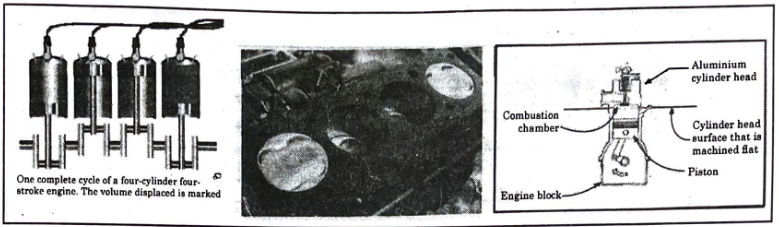
\includegraphics[width=\columnwidth]{figs/engine.png}
\caption{}
\label{fig:engine}
\end{figure}
 %use figure environment for inserting figure   

 \item The cylinder bore in the form of circular cylinder open at the top is to be made from a metal sheet of area ${75\pi}$ ${cm}^2.$ \\
Based on the above information , answer the following questions: 

 \begin{enumerate}[label=(\roman*)]

     \item  If the radius of cylinder is r cm and height is h cm, then write the volume V of cylinder in terms of radius r. 
     \item Find $\dfrac{dv}{dr}$ 
     
     \item 
	     \begin{enumerate}[label=(\alph*)]
     \item Find the radius of cylinder when its volume is maximum. 
   
     \item  For maximum volume, $h > r$.State true or false and justify. 
 \end{enumerate}
 \end{enumerate}

 \item The use of electric vehicles will curb air pollution in the long run.
 
\begin{figure}[H]
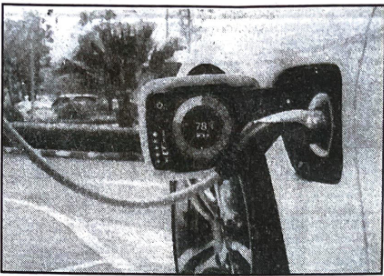
\includegraphics[width=\columnwidth]{figs/electricvehicle.png}
\caption{}
\label{fig:electricvehicle}
\end{figure}
  
 \item The use of electric vehicles is increasing every year and estimated electric vehicles in use at any time $t$ is given by the function $V$ :
 
 \begin{align}
    V\brak{t}=\frac{1}{5}t^3 - \frac{5}{2}t^2 + 25t-2 
 \end{align}
 Where $t$ represents the time and $t$=1,2,3\dots corresponds to year 2001,2002,2003\dots respectively.\\
 Based on the above information, answer the following questions :
 \begin{enumerate}[label=(\roman*)]
     \item Can the above function be used to estimate number of vehicles in the year 2000 ? Justify. 
     \item Prove that the function V\brak{t} is an increasing function.
 \end{enumerate}

\item The slope of the normal to the curve $y=2x^2+3\sin{x}$ at $x=0$ is \rule{30pt}{1pt}.

\item The total revenue (in \rupee) received from sale of x units of a product is $R(x)$ = $3x^2+36x+5$. The marginal revenue, when $x=12$ is \rule{30pt}{1pt}.

\item If $\sin y = x \sin(a+y)$, then prove that $\frac {dy}{dx} = \frac {\sin x^2(a+y)}{\sin a}$.

\item Find the equation of tangent to the curve $y=x^2+4x+1$ at the point(3,22).

\item If $Y = \tan^{-1}\left(\frac{3x - x^3}{1 - 3x^2}\right)$,-$\frac{1}{\sqrt{3}}$ \textless x \textless $\frac{1}{\sqrt{3}}$
then find $\frac{dy}{dx}$ and $\frac{{d^2y}}{{dx^2}}$.

\item If $\sec^{-1}\left(\frac{1+x}{1-y}\right)=a$, then $\frac{dy}{dx}$ is equal to

\item The oder and degree of the differential equation of the family of parabolas having at 
organ and axis along positive x-axis is

\item If $y = \log x$, then $\frac{{d^2y}}{{dx^2}}$=

\item Find the intervals in which the function f defined as $f(x) = \sin(x) + \cos(x)$,
$0 \leq x \leq 2\pi$ is strictly increasing or decreasing.

\item Prove that the radius of the right circular 
cylindar of greatest curved surface area which 
can be inscribed in a given cone is half of thatof the cone.

\item If $y=x^{\sin x }+\sin^{-1}(\sqrt x )$, the find $\frac{dy}{dx}$.

\item The supply function of a commodity is 
$100p = (x+20)^2$. Find the Producer's
Surplus(PS),whne the market price is \rupee 25.

\item Find:
$\int{\frac{2x^2 + 1}{x^2 - 3x + 2}}$dx

 \end{enumerate}







\chapter{Integration}
%\section{2010}
%\subsection{12}
%\begin{enumerate}
    \item Find: $\int \frac{1- \sin x}{\sin x (1 + \sin x)} dx$

    \item Find: $\int \sbrak{\log (\log x)+ \frac{1}{(\log x)^2}} dx$

    \item Evaluate: $\int_0^\frac{\pi}{2} \frac{\sin^2x}{\sin x + \cos x} dx$

    \item Evaluate : $ \int_0^1 \cot^{-1}\brak{1 - x + x^2} dx$

    \item Solve the differential equation: $(x + 1) \dfrac{dy}{dx} - y = e^{3x} (x + 1)^3$

    \item Solve the differential equation : $2y e^{\frac{x}{y}}dx + \brak{y - 2x e^{\frac{x}{y}}}dy = 0$

    \item Using integration find the area of the region ${(x, y) : y^2 \leq 6ax \text{ and }
                      x^2+y^2 \leq 16a^2}$.

    \item Find : $\int \frac{(2x-5)e^{2x}}{(2x-3)^3} dx$

    \item Find : $\int \frac{x^2 +x +1}{(x^2 + 1)(x + 2)} dx$

    \item Evaluate : $\int_{-2}^{2} \frac{x^2}{1+5^x} dx$

    \item Find : $\int (x+3)\sqrt{3 - 4x - x^2} dx$\\

    \item Find the particular solution of difference equation :\\
          \begin{align}
              \dfrac{dy}{dx} = - \frac{x + y\cos x}{1 + \sin x}
          \end{align}
          given that $y = 1$ when $x = 0$.

    \item Find the particualr solution of the differential equation
          \begin{align*}
              2y e^{\frac{x}{y}} dx + (y -2x e^{\frac{x}{y}}) dy = 0
          \end{align*}
          given that $x = 0$ when $y = 1$.

    \item Using the method of integration, find the area of the triangular region whose vertices are $(2, 2)$, $(4, 3)$ and $(1, 2)$.
    \item Evaluate : $\int_{0}^{\dfrac{3}{2}} \abs{x \cos \pi x}\,dx$
    \item Find: $\int \brak{3x +1}\sqrt{4-3x-2x^2} \,dx$.
    \item Using integration, find the area of the triangle formed by negative $x$-axis and tangent and normal to the circle
          \begin{align*}
              x^2 + y^2 =9
          \end{align*}
          at \brak{-1,2\sqrt{2}}
    \item Solve the differential equation
          \begin{align*}
              x\dfrac{dy}{dx} +y -x +xy \cot x= 0, \quad x\neq 0
          \end{align*}
    \item Solve the differential equation:
          \begin{align*}
              \brak{x^2+3xy+y^2}dx -x^2dy = 0
          \end{align*}
          given that $y=0$, when $x=1$.
    \item Find : $\int \brak{3x+5}\sqrt{5+4x-2x^2}\,dx$.
    \item Find : $\int \dfrac{2x+1}{\brak{x^2+1}\brak{x^2+4}}\,dx$.
    \item Evaluate : $\int_{0}^{\pi}\dfrac{x\sin x}{1+3\cos^2 x}\,dx$.
    \item Evaluate : $\int_{1}^{5}\cbrak{\abs{x-1}+\abs{x-2}+\abs{x-3}}\,dx$.
    \item Find :$\int \dfrac{x^2}{x^4 + x^2 -2}\,dx$.
    \item Evaluate : $\int_{0}^{\dfrac{\pi}{2}} \dfrac{\sin^2 x}{\sin x + \cos x} \,dx$.
    \item Solve the differential equation :
          \begin{align*}
              y+ x\dfrac{dy}{dx} = x-y\dfrac{dy}{dx}
          \end{align*}

    \item Find : $\int{\brak{3x+1}\sqrt{4 - 3x - 2x^2}dx}$
    \item Evaluate: $ \int^{\frac{\pi}{2}}_0{\dfrac{\sin^2{x}}{\sin{x} + \cos{x}}dx}$
    \item Evaluate: $\int^{\frac{3}{2}}_0{|x\cos{\pi x}|dx}$
    \item Find: $\int{\dfrac{x^2}{x^4 + x^2 -2}}$
    \item Evaluate: $\int^5_1{\abs{x-1} + \abs{x-2} + \abs{x-3} dx}$
    \item Evaluate: $ \int^{\pi}_0{\dfrac{x\sin{x}}{1 + 3\cos^2{x}}dx}$
    \item Find: $\int{\brak{3x+5}\sqrt{5 + 4x - 2x^2}dx}$
    \item Find: $\int{\dfrac{2x+1}{\brak{x^2 + 1}\brak{x^2 + 4}}dx}$
    \item Using integration, find the area of the triangle formed by the negative $x$-axis and tangent and normal to the circle $x^2 + y^2 = 9$ at $\brak{-1,2\sqrt{2}}$.
    \item Find: $\int{\brak{x+3}\sqrt{3 - 4x - x^2}dx}$.

    \item Find: $\int{\dfrac{(2x - 5)e^{2x}}{(2x-3)^3}dx}$

    \item Find: $\int{\dfrac{x^2+x+1}{(x^2+1)(x+2)}dx}$

    \item Evaluate: $\int_{-2}^{2}\dfrac{x^2}{1+5^x}dx$.

    \item Find the particular solution of differential equation: $\dfrac{dy}{dx} = -\dfrac{x+y\cos{x}}{1+\sin{x}}$ given that $y = 1$ when $x=0$.

    \item Using the method of integration, find the area of the triangular region whose vertices are $(2,-2), (4,-3)$ and $(1,2)$.
    \item Evaluate :
          \begin{align*}
              \int_{0}^\frac{\pi}{2}{\frac{\sin^2x}{\sin x+ \cos x}}{dx}
          \end{align*}
    \item Evaluate:
          \begin{align*}
              \int_{0}^\frac{3}{2}{\mydet{x \cos \pi x}}dx
          \end{align*}
    \item Find :
          \begin{align*}
              \int{\frac{x^2}{x^4+x^2-2}}dx
          \end{align*}
    \item Find : $\int{\brak{3x + 1} \sqrt{4-3x-2x^2}}dx $
    \item The equation of tangent at \brak{2,3} on the curve $y^2=ax^3+b$ is $y=3x-5$. Find the values of a and b.
    \item Find: $\int(x+3)\sqrt{3-4x-x^2} dx$.
    \item Evaluate: \(\int_{-2}^{2}\frac{x^2}{1+5^2}\,dx\).
    \item Find : $\int{\frac{(2x-5)e^{2x}}{(2x-3)^3}}dx$
    \item Find : $\int{\frac{x^2+x+1}{(x^2+1)(x+2)}}dx$
    \item Using the method of integration, find the area of the triangular region whose vertices are $(2, -2),(4,3)$ and $(1,2)$.
    \item Find :$ \int{\frac{2x+1}{(x^{2}+1)(x^{2}+4)}}dx$
    \item Evaluate: $\int{^5_1{|x-1|+|x-2|+|x-3|}dx}$
    \item Evaluate: $\int{^\pi_0\frac{xsinx}{1+3cos^{2}x}}dx$
    \item Find $\int(3x+5)\sqrt{5+4x-2x^{2}}dx$
    \item Using integration,find the area of the triangle formed by negative x-axis and tangent and normal to the circle $x^{2}+y^{2}=9$ at $(-1,2\sqrt{2})$.
    \item Find:$\int[log(logx)+\frac{1}{logx}^2]dx$
    \item Find: $\int\frac{1-sinx}{sinx(1+sinx)}dx$
    \item Evaluate: $ \int_{0}^{1}cot^{-1}(1-x+x^{2})dx$
    \item Find the equation of normal's to the curve $ay^{2}$=$x^{3}$ at the point whose x coordinate is a$m^{2}$.
    \item Using the integration find the area of the region
          $ (x,y):y^{2}<=6ax$ and $x^{2}+y^{2}<=16a^{2}$
    \item Evaluate: 
    \begin{align*}
        \int_0^\frac{\pi}{2} \frac{\sin^{2}x}{\sin x + \cos x} dx
    \end{align*}
    \item Evaluate:
    \begin{align*}
        \int_0^1 \cot^{-1}\brak{1 - x + x^{2}} dx
    \end{align*}
    \item Find: 
    \begin{align*}
        \int \sbrak{\log\brak{\log x} + \frac{1}{\brak{\log x}^{2}}} dx
    \end{align*}
    \item Find: 
    \begin{align*}
        \int \frac{1 - \sin x}{\sin x \brak{1 + \sin x}}dx
    \end{align*}
    \item Solve the differential equation: 
    \begin{align*}
        2y e^{\frac{x}{y}}dx + \brak{y - 2xe^{\frac{x}{y}}}dy = 0
    \end{align*}
    \item Solve the differential equation: 
    \begin{align*}
        \brak{x + 1} \frac{dy}{dx} - y = e^{3x}\brak{x + 1}^{3}
    \end{align*}
    \item Using integration, find the area of the region 
    \begin{align*}
        \cbrak{\brak{x,y} : y^{2} \leq 6ax, x^{2} + y^{2} \leq 16a^{2}}
    \end{align*}




\chapter{Functions}
%\section{2023}
%\subsection{12}
%%\documentclass{article}
%\usepackage{geometry}
%\usepackage{amsmath}%
%\providecommand{\abs}[1]{\lvert#1\rvert}
%\begin{document}
\begin{enumerate}
	\item The function $f(x) = x \abs{x} $ is
        \begin{enumerate}
            \item continuous and differentiable at $x$ = 0.
            \item continuous but not differentiable at $x$ = 0.
            \item differentiable but not continuous at $x$ = 0.
            \item neither differentiable nor continuous at $x$ = 0.
        \end{enumerate}
	 \item If
 	\begin{equation}
    	f(x) =  
    	\begin{cases}
            ax+b & 0<x \le 1 \\
            2x^2-x & 1<x<2
    	\end{cases}
 	\end{equation}
  	is a differentiable function is (0,2), then find the values of $a$ and $b$.
 	\item A function $ f: [-4,4] \rightarrow [0,4] $ is given by $ f(x) = \sqrt{16-x^2}$. Show that $f$ is an onto function but not a one-one                    function.Further,find all possible values of 'a' for which $ f(a) = \sqrt{7}.$
\end{enumerate}
%\end{document}

%\section{2014}
\begin{enumerate}
	\item Let $f$ be a one-to-one function from the set of natural numbers to itself such that $f\brak{mn} = f\brak{m} f\brak{n}$ for all natural numbers $m$ and $n$. What is the least possible value of $f\brak{999}$?\hfill(PRERMO 2014)
\end{enumerate}

%\section{chapters}
\begin{enumerate}
\item Let $N$ be the set of natural numbers. Suppose $f : N \rightarrow N$ is a function satisfying the following conditions:
    \begin{enumerate}
	    \item $f\brak{mn} = f\brak{m} f\brak{n}$,
	    \item $f\brak{m} < f\brak{n}$ if $m < n$,
	    \item $f\brak{2} = 2$.
    \end{enumerate}
	What is the value of $\sum_{k=1}^{20} f\brak{k}$ ?\hfill(PRERMO 2012)
	\item One is given a finite set of points in the plane, each point having integer coordinates. Is it always possible to color some of the points in the set red and the remaining points white in such a way that for any straight line $L$ parallel to either one of the coordinate axes the difference (in absolute value) between the numbers of white point and red points on $L$ is not greater than $1$?\hfill(IMO 1986)
\item Let $n$ be an integer greater than or equal to $2$. Prove that if $k^2+k+n$ is prime for all integers $k$ such that $0\leq k\leq \sqrt{n/3}$, then $k^2+k+n$ is prime for all integers $k$ such that $0\leq k\leq n-2$ \hfill(IMO 1987)
	\item A function $f$ is defined on the positive integers by
                  \begin{align*}
  f\brak{1}=1, f\brak{3}=3, \\
  f\brak{2n}=f\brak{n}, \\
                  f\brak{4n+1}=2f\brak{2n+1}-f\brak{n},\\
                  f\brak{4n+3}=3f\brak{2n+1}-2f\brak{n},\\ \end{align*}
                  for all positive integers n.
                  Determine the number of positive integers $n$, less than or equal to $1988$,for which $f(n) = n$.\hfill(IMO 1988)
                  \item Show that set of real numbers x which satisfy the in equality                                                                \begin{align*}\sum{k=1}^{70}\frac{k}{x-k}\geq \frac{5}{4}\\ \end{align*}                                                          is a union of disjoint intervals, the sum of whose lengths is $1988$\hfill(IMO 1988)
\item Let $Q^+$ be the set of positive rational numbers. Construct a function $ f: Q^+ \rightarrow Q^+$ such that 

			\begin{align*}  f\brak{xf\brak{y}}= \frac{f\brak{x}}{y} \end{align*}\\ for all $x , y$ in $Q^+$.\hfill(IMO 1990)


      \subsection*{COMBINATOMICS}

  \item Let $S = \{1,2,3,......,280\}$. Find the smallest integer $n$ such that each $n-$ element subset of $S$ contains five numbers which are pairwise relatively prime.\hfill(IMO 1991)

	  \subsection*{GRAPH THEORY}

  \item Suppose $G$ is a connected graph with $k$ edges. Prove that it is possible to label the edges $1,2.....k$ in such a way that at each vertex which belongs to two or more edges, the greatest common divisor of the integers labeling those edges is equal to $1$.
	  $[$ A graph consists of a set of points, called vertices, together with a set of edges joining certain pairs of distinct vertices. Each pair of vertices. $u, v$ belongs to at most one edge. The graph $G$ is connected if for cach pair of distinct vertices $x, y$ there is some sequence of vertices   $x=v_0,v_1,v_2,.......,v_m = y$  such that each pair $v_i,v_{i+1}\brak{0\leq i < m}$ is joined by an edge of G$.]$ \hfill(IMO 1991)
	  \item Let $Q^+$ be the set of positive rational numbers. Construct a function $ f: Q^+ \rightarrow Q^+$ such that 

			\begin{align*}  f\brak{xf\brak{y}}= \frac{f\brak{x}}{y} \end{align*}\\ for all $x , y$ in $Q^+$.\hfill(IMO 1990)
			\item Determine all functions $f: \textbf{R} \to \textbf{R}$ such that\\$f\brak{x - f\brak{y}} = f\brak{f\brak{y}} + xf\brak{y} + f\brak{x} - 1$ \\for all real numbers x,y.\hfill(IMO 1999)
			\item Determine all functions $f:R \rightarrow R $ such that the euality
				\begin{align}
					f(\lfloor{x} \rfloor{y})=f(x) \lfloor{f(y)} \rfloor
				\end{align}
				holds for all $x,y \in R $.(Here $\lfloor{z}\rfloor$ denotes the greatest integer less than or equal to $z$.)\hfill(IMO2010)
			\item Let $f:R \rightarrow R$ be a real-valued function defined on the set of real numbers that satisfies
				\begin{align}
					f\brak x+y \leq{y f\brak x}+f\brak{f\brak x}
				\end{align}
				for all real numbers $x$ and $y$. Prove that $f \brak x=0$ for all $x\leq{0}$.\hfill(IMO2011)
			\item Let $n>0$ be an integer. We are given a balance and $n$ weights of weight $2^{0}, 2^{1}, \dots, 2^{n-1}$. We are to place each of the $n$ weights on the balance, one after another, in such way that the right pan is never heavier than the left pan. At each step we choose one of the weights that has not yet been placed on the balance, and place it on either the left pan or the right pan, unwtil all of the weights have been placed.
				Determine the number of ways in which this can be done.\hfill(IMO2011)
			\item The liar's guessing game is a game played between two players $A$ and $B$. The rules of the game depend on two positive integers $k$ and $n$ which are known to both players. At the start of the game$A$ chooses integers $x$ and $N$ with $1\leq{x}\leq{N}$. Player $A$ keeps $x$ secret, and truthfully tells $N$ to player $B$. Player $B$ now tries to obtain information about $x$ by asking player $A$ questions as follows: each question consists of $B$ specifying an arbitrary set $S$ of positive integers (possibly one specified in some previous question), and asking $A$ whether $x$ belongs to $S$. Player $B$ may ask as many such questions as he wishes. After each question, player $A$ must immediately answer it with yes or no, but is allowed to lie as many times as she wants; the only restriction is that, among any $k + 1$ consecutive answers, at least one answer must be truthful.
				After $B$ has asked as many questions as he wants, he must specify a set $X$ of at most $n$ positive integers. If $x$ belongs to $X$, then $B$ wins; otherwise, he loses. Prove that:
				1. If $n\geq{2^{k}}$, then $B$ can guarantee a win.
				2. For all sufficiently large $k$, there exists an integer $n\geq{1.99^{k}}$ such that $B$ cannot guarantee a win.\hfill(IMO2012)
			\item  Find all positive integers $n$ for which there exist non-negative integers $a_{1}, a_{2}, \dots, a_{n}$ such that
				\begin{align}
					\frac{1}{2^{a_{1}}}+\frac{1}{2^{a_{2}}}+ \dots +\frac{1}{2^{a_{n}}}=\frac{1}{3^{a_{1}}}+\frac{1}{3^{a_{2}}}+ \dots +\frac{n}{3^{a_{n}}}=1.\hfill(IMO2012)
				\end{align}

\end{enumerate}


\chapter{Matrices}
%\section{2020}
%\subsection{10}
\begin{enumerate}
\item A $n\times n$ matrix whose entires come from the set $S = \cbrak{1,2,\dots,2n-1}$ is called a silver matrix if, for each ${i=1,2,\dots,n,}$ the ith row and ith column together contain all elements of $S$. Show that                                     
\begin{enumerate}                        
	\item there is no silver matrix for $n=1997$;      
\item silver matrices exist for infinitely many values of $n$.\hfill(IMO 1997) 
\end{enumerate}
\item The positive integers $a$ and $b$ are such that the numbers $15a+16b$ and $16a-15b$ are both squares of positive integers. What is the least possible value that can be taken on by the smaller of these two squares?\hfill(IMO 1996)
\end{enumerate}	




\chapter{Trignometry}
%\section{2019}
%\subsection{10}
%\begin{enumerate}

\item A boy standing on a horizontal plane finds a bird flying at a distance of $100 m$ from him at an elevation of $30\degree$. A girl standing on the roof of a $20 m$ high building, finds the elevation of the same bird to be $45\degree$. The boy and the girl are on the opposite sides of the bird. Find the distance of the bird from the girl. (Given ${\sqrt 2}= 1.414$)

\item The angle of elevation of an aeroplane from a point $A$ on the ground is $60\degree$. After a flight of $30 $seconds , the angle of elevation changes to $30\degree$. If the plane is flying at a constant height of $3600\sqrt 3 $ metres, find the speed of the aeroplane.

\end{enumerate}

%\section{2014}
\begin{enumerate}
\item In a triangle $ABC$, let $I$ denote the incenter. Let the lines $AI$, $BI$, and $CI$ intersect the incircle at $P$, $Q$, and $R$, respectively. If $\angle BAC = 40\degree$, what is the value of $\angle QPR$ in degrees?\hfill(PRERMO 2014)
\item Four real constants $a, b, A, B$ are given, and \begin{align}
f\brak{\theta} = 1 - a\cos\theta - b \sin \theta     - A \cos 2\theta - B \sin 2\theta  
\end{align}. Prove that if 
\begin{align}f\brak{\theta} \textgreater= 0 
	\end{align} ,for all real $\theta$, then
\begin{align} a^{2} + b^{2} \leq 2 and A^{2} + B^{2} \geq = 1 
\end{align}\hfill(Imo 1977)

		
	

\end{enumerate}



%\include{ch02} 
\backmatter
\appendix
\iffalse
\chapter{Conic Lines}
\section{Pair of Straight Lines}
%
\input{quad/pair.tex}
\section{Intersection of Conics}
\input{quadlines/inter.tex}
\section{ Chords of a Conic}
\input{quadlines/chord.tex}
\section{ Tangent and Normal}
The equation of the {\em incircle} is given by 
		\begin{align}
			\label{eq:incircle}
			\norm{\vec{x}-\vec{O}}^2 = r^2
		\end{align}
		which can be expressed as 
			 \eqref{eq:conic_quad_form}
			 using 
			 \eqref{eq:conic_quad_form-params}.
	In \figref{fig:incircle}, 
Let 
  \eqref{eq:line_dir_pt-lam}
  be the equation of $AB$.  Then, the intersection of 
  \eqref{eq:line_dir_pt-lam}
  and 
			 \eqref{eq:conic_quad_form}
			 can be expressed as 
\begin{align}
\brak{\vec{h} + \mu{\vec{m}}}^{\top}
\vec{V}
\brak{\vec{h} + \mu{\vec{m}}}
			+2\vec{u}^{\top}\brak{\vec{h} + \mu{\vec{m}}}+f &= 0
			\\
\implies \mu^2\vec{m}^{\top} \vec{V}\vec{m} + 2\mu \vec{m}^{\top}\brak{\vec{V}\vec{h}+\vec{u}}+g\brak{\vec{h}} &= 0 
	\label{eq:incircle-quad}
\end{align}
For 	\eqref{eq:incircle-quad} to have exactly one root, the discriminant
\begin{align}
 \cbrak{\vec{m}^{\top}\brak{\vec{V}\vec{h}+\vec{u}}}^2 -g\brak{\vec{h}}\vec{m}^{\top} \vec{V}\vec{m}  &= 0 
	\label{eq:incircle-disc}
\end{align}
and 
  \eqref{eq:line_dir_pt-lam-mu}
  is obtained.
	\eqref{eq:incircle-disc}
	can be expressed as
\begin{align}
\vec{m}^{\top}\brak{\vec{V}\vec{h}+\vec{u}}^{\top}\brak{\vec{V}\vec{h}+\vec{u}}\vec{m}-g\brak{\vec{h}}\vec{m}^{\top} \vec{V}\vec{m}  &= 0 
\\
\implies \vec{m}^{\top}\vec{\Sigma}\vec{m} &= 0
	\label{eq:incircle-disc-Sigma-new}
\end{align}
for $\vec{\Sigma}$ defined in 
	\eqref{eq:incircle-disc-Sigma-new}.
      Substituting \eqref{eq:conic_parmas_eig_def}
	in \eqref{eq:incircle-disc-Sigma-new},
\begin{align}
\vec{m}^{\top}\vec{P}\vec{D}\vec{P}^{\top}\vec{m} &= 0
\\
\implies 
\vec{v}^{\top}\vec{D}\vec{v} &= 0
	\label{eq:incircle-disc-v}
\end{align}
where 
\begin{align}
	\label{eq:incircle-disc-v-lam-P}
\vec{v} = \vec{P}^{\top}\vec{m}
\end{align}
	\eqref{eq:incircle-disc-v}
	can be expressed as 
\begin{align}
\lambda_1 v_1^2
-\lambda_2 v_2^2 &= 0
\\
\implies \vec{v} = \myvec{\sqrt{\abs{\lambda_2}} \\[2mm]  \pm \sqrt{\abs{\lambda_1}}}
	\label{eq:incircle-disc-v-lam}
\end{align}
after some algebra.
From 
	\eqref{eq:incircle-disc-v-lam}
	and
	\eqref{eq:incircle-disc-v-lam-P}
	we obtain 
	  \eqref{eq:h-tangents-cond-mPlam}.

\fi
%\chapter{Proofs}
%   \section{}
%\input{apps/defs.tex}

%  \section{}
%\input{apps/parab.tex}
%  \section{}
%\input{apps/nonparab.tex}
%		\section{}
%\input{apps/params.tex}
\latexprintindex

\end{document}

 
\section{Examples}
\subsection{Loney}
\input{examples/loney.tex}
\subsection{Miscellaneous}
%\documentclass{exam}
%\usepackage{float}
%\usepackage{array}
%\usepackage{enumitem}
%\usepackage{amsmath}
%\begin{document}
\begin{enumerate}
	
	\item Find the distance of the point $(1,-2,9)$ from the point of intersection of the line
		\begin{align}
			\vec{r}=4\hat{i}+2\hat{j}+7\hat{k}+\lambda(3\hat{i}+4\hat{j}+2\hat{k})
		\end{align}and the plane
		\begin{align}
			\vec{r}\cdot(\hat{i}-\hat{j}+\hat{k})=10.
		\end{align}

	\item Find the area bounded by the curves $y=\abs{x-1}$ and $y=1$, using integration.

	\item Find the coordinates of the point where the line through $(4,-3,-4)$ and $(3,-2,2)$ crosses the plane $2x+y+z=6$.

	\item Fit a straight line trend by the method of least squares and find the trend value for the year 2008 using the data from Table \ref{tab:LC}:
		\begin{table}[H]
			\caption{Table showing yearly trend of production of goods in lakh tonnes \label{tab:LC}}
			%%%%%%%%%%%%%%%%%%%%%%%%%%%%%%%%%%%%%%%%%%%%%%%%%%%%%%%%%%%%%%%%%%%%%%
%%                                                                  %%
%%  This is the header of a LaTeX2e file exported from Gnumeric.    %%
%%                                                                  %%
%%  This file can be compiled as it stands or included in another   %%
%%  LaTeX document. The table is based on the longtable package so  %%
%%  the longtable options (headers, footers...) can be set in the   %%
%%  preamble section below (see PRAMBLE).                           %%
%%                                                                  %%
%%  To include the file in another, the following two lines must be %%
%%  in the including file:                                          %%
%%        \def\inputGnumericTable{}                                 %%
%%  at the beginning of the file and:                               %%
%%        \input{name-of-this-file.tex}                             %%
%%  where the table is to be placed. Note also that the including   %%
%%  file must use the following packages for the table to be        %%
%%  rendered correctly:                                             %%
%%    \usepackage[latin1]{inputenc}                                 %%
%%    \usepackage{color}                                            %%
%%    \usepackage{array}                                            %%
%%    \usepackage{longtable}                                        %%
%%    \usepackage{calc}                                             %%
%%    \usepackage{multirow}                                         %%
%%    \usepackage{hhline}                                           %%
%%    \usepackage{ifthen}                                           %%
%%  optionally (for landscape tables embedded in another document): %%
%%    \usepackage{lscape}                                           %%
%%                                                                  %%
%%%%%%%%%%%%%%%%%%%%%%%%%%%%%%%%%%%%%%%%%%%%%%%%%%%%%%%%%%%%%%%%%%%%%%



%%  This section checks if we are begin input into another file or  %%
%%  the file will be compiled alone. First use a macro taken from   %%
%%  the TeXbook ex 7.7 (suggestion of Han-Wen Nienhuys).            %%
\def\ifundefined#1{\expandafter\ifx\csname#1\endcsname\relax}


%%  Check for the \def token for inputed files. If it is not        %%
%%  defined, the file will be processed as a standalone and the     %%
%%  preamble will be used.                                          %%
\ifundefined{inputGnumericTable}

%%  We must be able to close or not the document at the end.        %%
 \def\gnumericTableEnd{\end{document}}


%%%%%%%%%%%%%%%%%%%%%%%%%%%%%%%%%%%%%%%%%%%%%%%%%%%%%%%%%%%%%%%%%%%%%%
%%                                                                  %%
%%  This is the PREAMBLE. Change these values to get the right      %%
%%  paper size and other niceties.                                  %%
%%                                                                  %%
%%%%%%%%%%%%%%%%%%%%%%%%%%%%%%%%%%%%%%%%%%%%%%%%%%%%%%%%%%%%%%%%%%%%%%

 \documentclass[12pt%
     %,landscape%
                    ]{report}
       \usepackage[latin1]{inputenc}
       \usepackage{fullpage}
       \usepackage{color}
       \usepackage{array}
       \usepackage{longtable}
       \usepackage{calc}
       \usepackage{multirow}
       \usepackage{hhline}
       \usepackage{ifthen}

 \begin{document}


%%  End of the preamble for the standalone. The next section is for %%
%%  documents which are included into other LaTeX2e files.          %%
\else

%%  We are not a stand alone document. For a regular table, we will %%
%%  have no preamble and only define the closing to mean nothing.   %%
    \def\gnumericTableEnd{}

%%  If we want landscape mode in an embedded document, comment out  %%
%%  the line above and uncomment the two below. The table will      %%
%%  begin on a new page and run in landscape mode.                  %%
%       \def\gnumericTableEnd{\end{landscape}}
%       \begin{landscape}


%%  End of theelse clause for this file being \input.              %%
\fi

%%%%%%%%%%%%%%%%%%%%%%%%%%%%%%%%%%%%%%%%%%%%%%%%%%%%%%%%%%%%%%%%%%%%%%
%%                                                                  %%
%%  The rest is the gnumeric table, except for the closing          %%
%%  statement. Changes below will alter the table's appearance.     %%
%%                                                                  %%
%%%%%%%%%%%%%%%%%%%%%%%%%%%%%%%%%%%%%%%%%%%%%%%%%%%%%%%%%%%%%%%%%%%%%%

\providecommand{\gnumericmathit}[1]{#1} 
%%  Uncomment the next line if you would like your numbers to be in %%
%%  italics if they are italizised in the gnumeric table.           %%
%\renewcommand{\gnumericmathit}[1]{\mathit{#1}}
\providecommand{\gnumericPB}[1]%
{\let\gnumericTemp=\\#1\let\\=\gnumericTemp\hspace{0pt}}
 \ifundefined{gnumericTableWidthDefined}
        \newlength{\gnumericTableWidth}
        \newlength{\gnumericTableWidthComplete}
        \newlength{\gnumericMultiRowLength}
        \global\def\gnumericTableWidthDefined{}
 \fi
%% The following setting protects this code from babel shorthands.  %%
 \ifthenelse{\isundefined{\languageshorthands}}{}{\languageshorthands{english}}
%%  The default table format retains the relative column widths of  %%
%%  gnumeric. They can easily be changed to c, r or l. In that case %%
%%  you may want to comment out the next line and uncomment the one %%
%%  thereafter                                                      %%
\providecommand\gnumbox{\makebox[0pt]}
%%\providecommand\gnumbox[1][]{\makebox}

%% to adjust positions in multirow situations                       %%
\setlength{\bigstrutjot}{\jot}
\setlength{\extrarowheight}{\doublerulesep}

%%  The \setlongtables command keeps column widths the same across  %%
%%  pages. Simply comment out next line for varying column widths.  %%
\setlongtables

\setlength\gnumericTableWidth{%
 53pt+%
 53pt+%
 106pt+%
0pt}
\def\gumericNumCols{3}
\setlength\gnumericTableWidthComplete{\gnumericTableWidth+%
         \tabcolsep*\gumericNumCols*2+\arrayrulewidth*\gumericNumCols}
\ifthenelse{\lengthtest{\gnumericTableWidthComplete > \linewidth}}%
         {\def\gnumericScale{\ratio{\linewidth-%
                        \tabcolsep*\gumericNumCols*2-%
                        \arrayrulewidth*\gumericNumCols}%
{\gnumericTableWidth}}}%
{\def\gnumericScale{1}}

%%%%%%%%%%%%%%%%%%%%%%%%%%%%%%%%%%%%%%%%%%%%%%%%%%%%%%%%%%%%%%%%%%%%%%
%%                                                                  %%
%% The following are the widths of the various columns. We are      %%
%% defining them here because then they are easier to change.       %%
%% Depending on the cell formats we may use them more than once.    %%
%%                                                                  %%
%%%%%%%%%%%%%%%%%%%%%%%%%%%%%%%%%%%%%%%%%%%%%%%%%%%%%%%%%%%%%%%%%%%%%%

\ifthenelse{\isundefined{\gnumericColA}}{\newlength{\gnumericColA}}{}\settowidth{\gnumericColA}{\begin{tabular}{@{}p{53pt*\gnumericScale}@{}}x\end{tabular}}
\ifthenelse{\isundefined{\gnumericColB}}{\newlength{\gnumericColB}}{}\settowidth{\gnumericColB}{\begin{tabular}{@{}p{150pt*\gnumericScale}@{}}x\end{tabular}}
\ifthenelse{\isundefined{\gnumericColC}}{\newlength{\gnumericColC}}{}\settowidth{\gnumericColC}{\begin{tabular}{@{}p{106pt*\gnumericScale}@{}}x\end{tabular}}

\begin{longtable}[c]{%
 b{\gnumericColA}%
 b{\gnumericColB}%
 b{\gnumericColC}%
 }

%%%%%%%%%%%%%%%%%%%%%%%%%%%%%%%%%%%%%%%%%%%%%%%%%%%%%%%%%%%%%%%%%%%%%%
%%  The longtable options. (Caption, headers... see Goosens, p.124) %%
% \caption{The Table Caption.}             \\ %
% \hline % Across the top of the table.
%%  The rest of these options are table rows which are placed on    %%
%%  the first, last or every page. Use \multicolumn if you want.    %%

%%  Header for the first page.                                      %%
% \multicolumn{3}{c}{The First Header} \\ \hline 
% \multicolumn{1}{c}{colTag} %Column 1
% &\multicolumn{1}{c}{colTag} %Column 2
% &\multicolumn{1}{c}{colTag} \\ \hline %Last column
% \endfirsthead

%%  The running header deinition.

%%
% \hline
% \multicolumn{3}{l}{\ldots\small\slshape continued} \\ \hline
% \multicolumn{1}{c}{colTag} %Column 1
% &\multicolumn{1}{c}{colTag} %Column 2
% &\multicolumn{1}{c}{colTag} \\ \hline %Last column
% \endhead

%%  The running footer definition.                                  %%
% \hline
% \multicolumn{3}{r}{\small\slshape continued\ldots} \\
% \endfoot

%%  The ending footer definition.                                   %%
% \multicolumn{3}{c}{That's all folks} \\ \hline 
% \endlastfoot
%%%%%%%%%%%%%%%%%%%%%%%%%%%%%%%%%%%%%%%%%%%%%%%%%%%%%%%%%%%%%%%%%%%%%%

\hhline{|-|-|-}
  \multicolumn{1}{|p{\gnumericColA}|}%
 {\gnumericPB{\raggedright}\gnumbox[l]{Year}}
 &\multicolumn{1}{p{\gnumericColB}|}%
	{\gnumericPB{\raggedright}\gnumbox[l]{Production (in lakh tonnes)}}
 %&\multicolumn{1}{p{\gnumericColC}|}%
 %{\gnumericPB{\raggedright}\gnumbox[l]{Description}}
\\
\hhline{|---|}
  \multicolumn{1}{|p{\gnumericColA}|}%
 {\gnumericPB{\raggedright}\gnumbox[l]{2001}}
 &\multicolumn{1}{p{\gnumericColB}|}%
 {\gnumericPB{\raggedright}\gnumbox[l]{30}}
 %&\multicolumn{1}{p{\gnumericColC}|}%
 %{\gnumericPB{\raggedright}\gnumbox[l]{Vertex A}}
\\
\hhline{|---|}
  \multicolumn{1}{|p{\gnumericColA}|}%
 {\gnumericPB{\raggedright}\gnumbox[l]{2002}}
 &\multicolumn{1}{p{\gnumericColB}|}%
 {\gnumericPB{\raggedright}\gnumbox[l]{35}}
 %&\multicolumn{1}{p{\gnumericColC}|}%
 %{\gnumericPB{\raggedright}\gnumbox[l]{Vertex B}}
\\
\hhline{|---|}
  \multicolumn{1}{|p{\gnumericColA}|}%
 {\gnumericPB{\raggedright}\gnumbox[l]{2003}}
 &\multicolumn{1}{p{\gnumericColB}|}%
 {\gnumericPB{\raggedright}\gnumbox[l]{36}}
 %&\multicolumn{1}{p{\gnumericColC}|}%
 %{\gnumericPB{\raggedright}\gnumbox[l]{Vertex C}}
\\
\hhline{|---|}
  \multicolumn{1}{|p{\gnumericColA}|}%
 {\gnumericPB{\raggedright}\gnumbox[l]{2004}}
 &\multicolumn{1}{p{\gnumericColB}|}%
 {\gnumericPB{\raggedright}\gnumbox[l]{32}}
 %&\multicolumn{1}{p{\gnumericColC}|}%
 %{\gnumericPB{\raggedright}\gnumbox[l]{Midpoint of AC}}
\\
\hhline{|---|}
  \multicolumn{1}{|p{\gnumericColA}|}%
 {\gnumericPB{\raggedright}\gnumbox[l]{2005}}
 &\multicolumn{1}{p{\gnumericColB}|}%
 {\gnumericPB{\raggedright}\gnumbox[l]{37}}
 %&\multicolumn{1}{p{\gnumericColC}|}%
 %{\gnumericPB{\raggedright}\gnumbox[l]{Midpoint of BC}}
\\
\hhline{|---|}
  \multicolumn{1}{|p{\gnumericColA}|}%
 {\gnumericPB{\raggedright}\gnumbox[l]{2006}}
 &\multicolumn{1}{p{\gnumericColB}|}%
 {\gnumericPB{\raggedright}\gnumbox[l]{40}}
 %&\multicolumn{1}{p{\gnumericColC}|}%
 %{\gnumericPB{\raggedright}\gnumbox[l]{Midpoint of AB}}
\\
\hhline{|-|-|-|}
\end{longtable}

\ifthenelse{\isundefined{\languageshorthands}}{}{\languageshorthands{\languagename}}
\gnumericTableEnd

		\end{table}
\end{enumerate}
%\end{document}

%
%%\section*{Disclosure Statement}
%%The authors report there are no competing interests to declare.
%%
%%
%%
%%  
%%%All the results related to conics are summarized in 
%%%Table \ref{table:conics}.  
%%%\begin{table*}[!t]
%%%\centering
%%%\input{conics.tex}
%%%%\input{./figs/conics.tex}
%%%\caption{$\vec{x}^{\top}\vec{V}\vec{x}+2\vec{u}^{\top}\vec{x}+f = 0$  can be expressed in the above standard form for various conics. $\vec{c}$ represents the centre/vertex of the conic. $\vec{q}$ is/are the point(s) of contact for the tangent(s). }
%%%\label{table:conics}
%%%\end{table*}
%%%\begin{verbatim}
%%\bibliographystyle{tfs}
%%%\bibliography{interacttfssample}
%%\bibliography{school}
%%\end{verbatim}
%% included where the list of references is to appear, where \texttt{tfs.bst} is the name of the \textsc{Bib}\TeX\ bibliography style file for Taylor \& Francis' Reference Style S and \texttt{interacttfssample.bib} is the bibliographic database included with the \textsf{Interact}-TFS \LaTeX\ bundle (to be replaced with the name of your own .bib file). \LaTeX/\textsc{Bib}\TeX\ will extract from your .bib file only those references that are cited in your .tex file and list them in the References section.
%
%% Please include a copy of your .bib file and/or the final generated .bbl file among your source files if your .tex file does not contain a reference list in a \texttt{thebibliography} environment.
%

  % \section{Appendices}
  % \appendix

\appendices
